\chapter{Custom Data Types} % (fold)
\label{cha:more_data_types}

\begin{quote}
  \Fontlukas\Large
  \renewcommand{\LettrineTextFont}{\relax}
  \lettrine[image=true,lines=3,lraise=0.1]
  {Y}{ou} are progressing well! You have learnt to structure your spells, guide the flow of magic, and apply it to many targets. Now it is time to see how you can also structure the components that go into your spells. Fetch the snake and dragon scale, now turn your thoughts to their structure. Take your wand and\ldots
\end{quote}

\bigskip


\cref{cha:managing_multiple_values} introduced the array, allowing you to store multiple values of the same type in a single variable. This greatly expanded the ways in which you can work with data in your code, but there are more tools you can use to model data in your programs.

This chapter will show you how to create your own data types, allowing you to model the entities\footnote{A fancy way of saying the `\emph{things}' associated with your program.} related to your program. This means that your code can work with more meaningful values, making it easier to create larger and more complicated programs.

When you have understood the material in this chapter you will be able to define your own data types to model the entities you want to work with in your program.

\minitoc

% ============
% = Concepts =
% ============
\clearpage
\section{Custom Data Type Concepts} % (fold)
\label{sec:data_type_concepts}

To this point, data has been about single values that are either numbers, text, or Boolean values. These values can be used in \nameref{sub:expression}s and stored in \nameref{sub:variable}s and \nameref{sub:array} elements. Now as we move to creating larger and more complicated programs you need a more effective means of modelling the data in your code. This chapter introduces concepts that you can use to more accurately model the data and entities associated with your program.

This chapter introduces the following \textbf{artefacts}:
\begin{itemize}
  \item \nameref{ssub:enum}: a kind of type used to store one of a list of available options.
  \item \nameref{ssub:record}: a kind of type used to store multiple fields in a single composite value.
  \item \nameref{ssub:union}: a kind of type used to store one value of different possible types.
\end{itemize}

\bigskip

You may need to revise the following programming artefacts:
\begin{itemize}
  \item \nameref{sub:variable}: The idea of storing data within your code.
  \item \nameref{sub:array}: Allowing you to store multiple values within your code.
  \item \nameref{sub:local_variable}: Storing data in a \nameref{sub:function} or \nameref{sub:procedure}.
  \item \nameref{sub:parameter}: Passing data to a Function or Procedure.
\end{itemize}

The following programming terminology will also be used in this Chapter:
\begin{itemize}
  \item \nameref{sub:expression}: A value used in a statement.
  \item \nameref{sub:type}: A kind of data used in your code.
\end{itemize}

The example program for this chapter will be Small DB, a program that allows the user to enter a number of integer, double, and text values.

\begin{figure}[h]
   \centering
   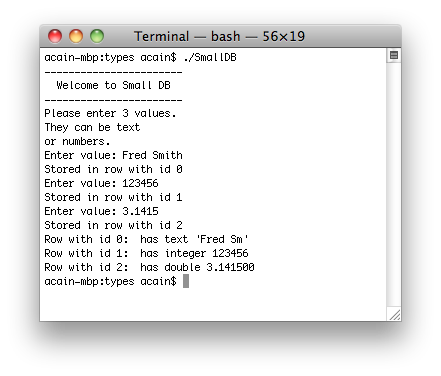
\includegraphics[width=0.7\textwidth]{./topics/type-decl/images/SmallDB} 
   \caption{Small DB run from the Terminal}
   \label{fig:small-db}
\end{figure}


\clearpage
\subsection{Type (recap)} % (fold)
\label{sub:type_recap_}

This chapter is all about types, so its is important to have a good understanding of what a type is. A type is a specification for a class of data, describing how it is stored and interpreted.

\begin{figure}[h]
   \centering
   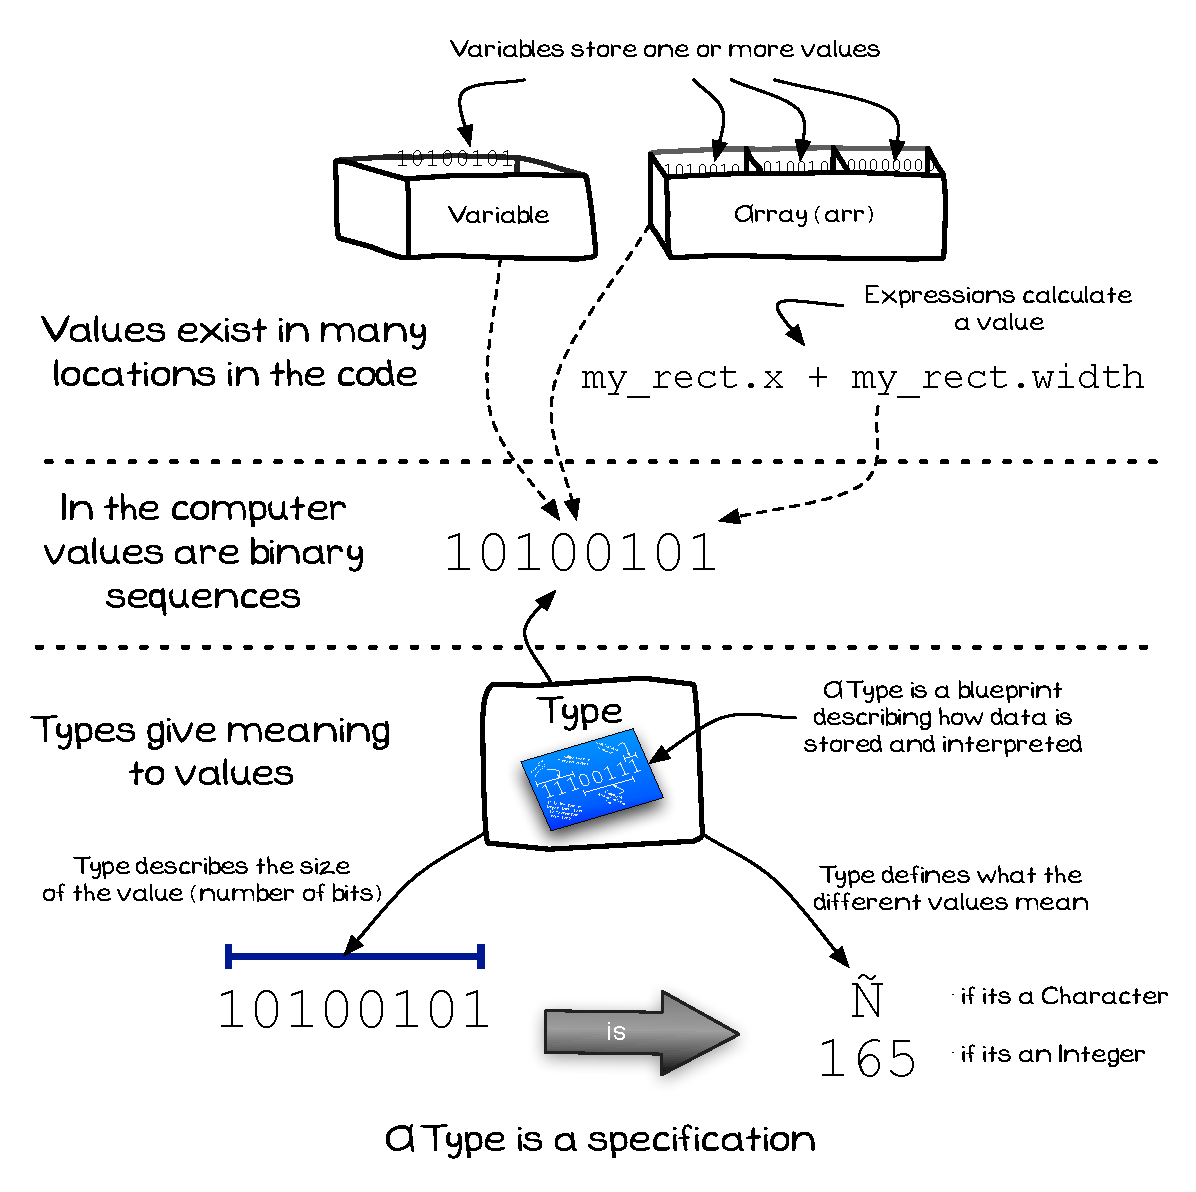
\includegraphics[width=\textwidth]{./topics/type-decl/diagrams/TypeRecap} 
   \caption{Type defines the size and interpretation if values in your code}
   \label{fig:type-recap}
\end{figure}

\mynote{
\begin{itemize}
  \item A Type is a kind of \texttt{artefact}, describing the format and interpretation of values.
  \item Types specify the following:
  \begin{itemize}
    \item The size (number of bits) needed to store values of this type.
    \item How the bits of the type are interpreted.
    \item The operations that can be performed on values of this type.
  \end{itemize}
  \item You can think of a Type as a blueprint, specifying data layout.
  \item The interpretation of a value depends on its Type, for example \texttt{10100101} is \~{N} if the value is a Character type, but the same value would be \texttt{165} if it is an Integer type.
  \item You can create your own types...
\end{itemize}
}

% subsection type_recap_ (end)
\clearpage
\subsection{Program (with Type Declarations)} % (fold)
\label{sub:program_with_type_declarations_}

\begin{figure}[h]
   \centering
   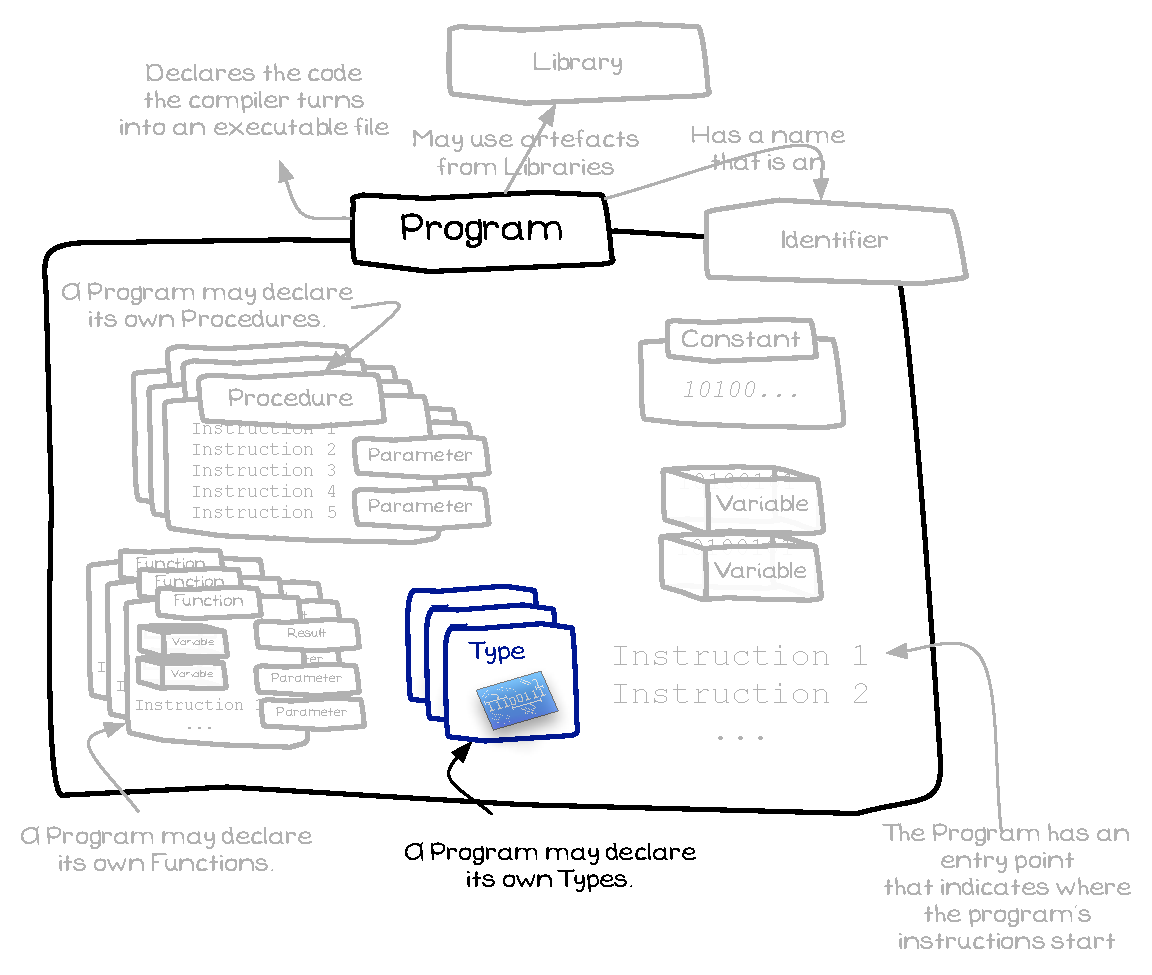
\includegraphics[width=\textwidth]{./topics/type-decl/diagrams/ProgramWithTypes} 
   \caption{A Program can contain Type Declarations}
   \label{fig:type-decl-program}
\end{figure}

% subsection program_with_type_declarations_ (end)
\clearpage
\subsection{Type Declaration} % (fold)
\label{sub:type_declaration}

\begin{figure}[h]
   \centering
   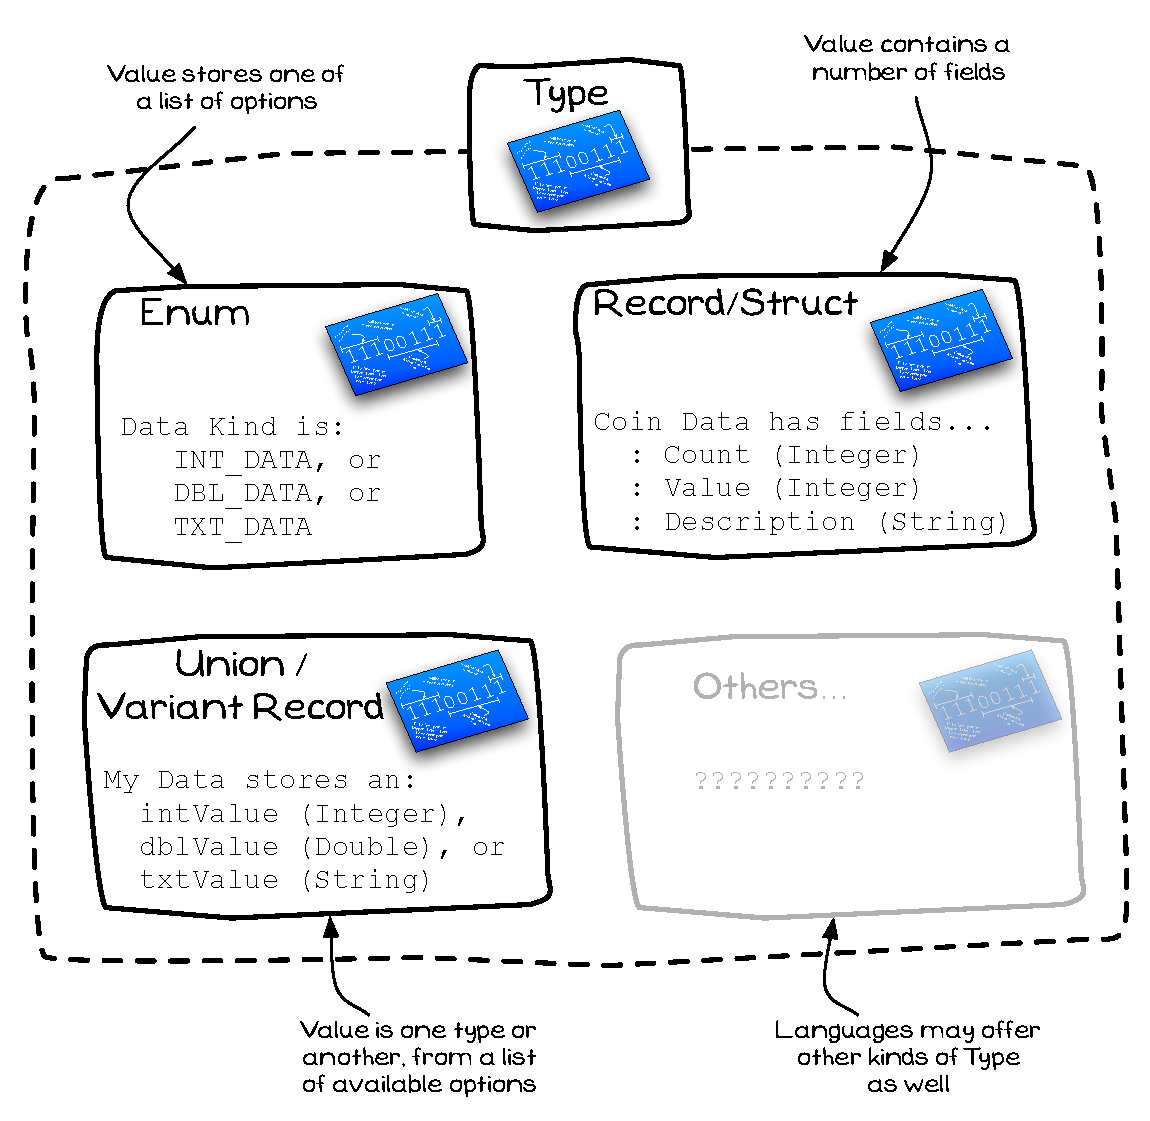
\includegraphics[width=\textwidth]{./topics/type-decl/diagrams/TypeDecl} 
   \caption{You can declare your own Data Types}
   \label{fig:type-decl-type-decl}
\end{figure}

% subsection type_declaration (end)
\clearpage
\subsection{Declaring Variables (with custom types)} % (fold)
\label{sub:declaring_variables_with_custom_types_}

The custom types allow you to specify a data format. To make use of this format you must declare variables that use this type. The type can be used to declare \nameref{sub:local_variable}s and \nameref{sub:parameter}s, allowing you to store values in this format and pass the around between your functions and procedures.

\begin{figure}[h]
   \centering
   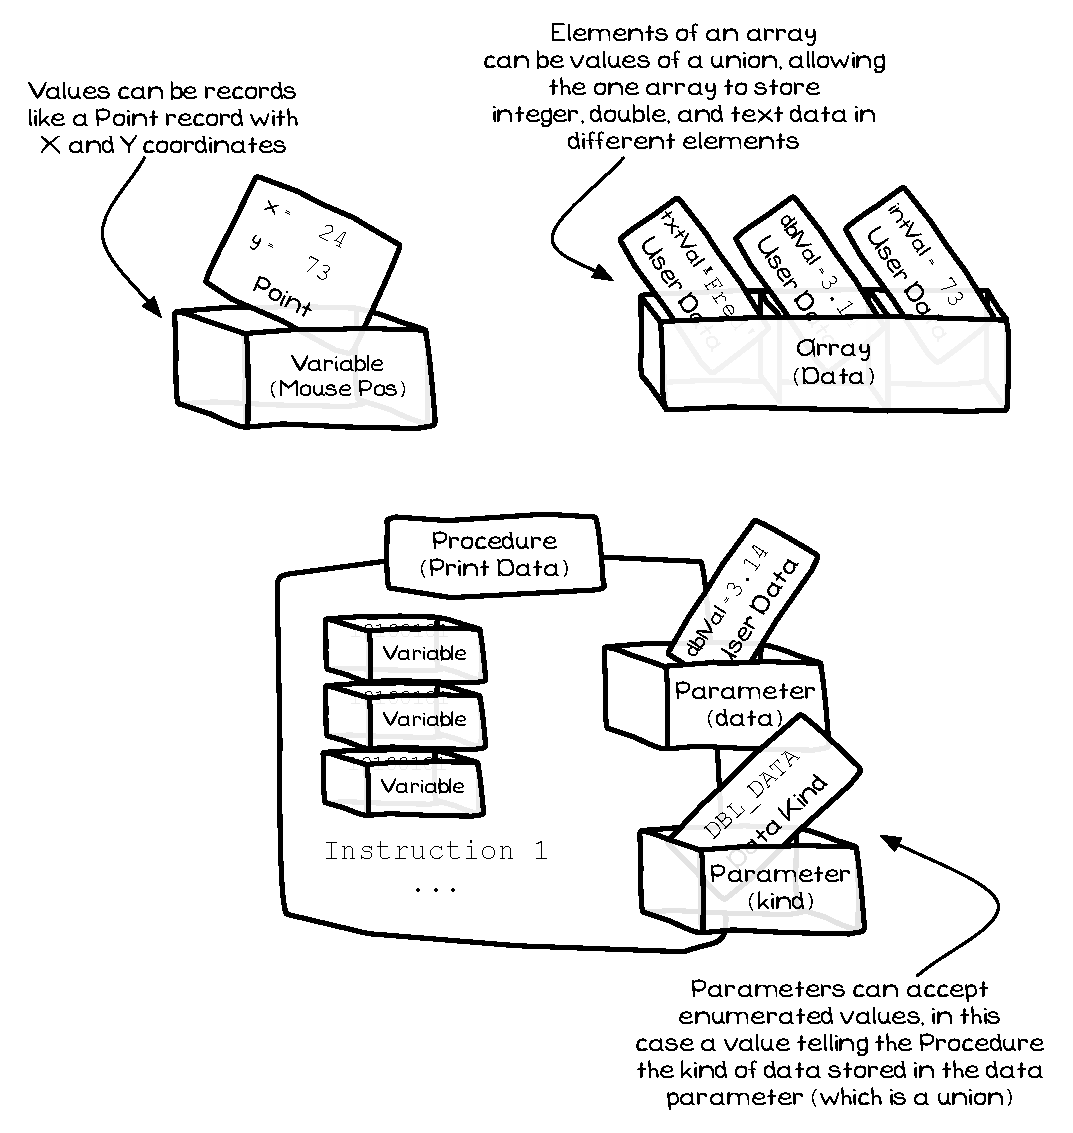
\includegraphics[width=0.87\textwidth]{./topics/type-decl/diagrams/VariableDeclaration} 
   \caption{Some examples of how you can use your types to declare the kind of data stored in variables}
   \label{fig:type-decl-variable-decl}
\end{figure}

\mynote{
\begin{itemize}
  \item Variables declaration is the \textbf{term} given to the code that creates Variables.
  \item The Variables you create store data as described in your custom type definitions.
  \item In \fref{fig:type-decl-variable-decl} there are the following examples:
  \begin{itemize}
    \item \texttt{Mouse Pos}: A Variable that stores \texttt{Point} \nameref{ssub:record} data.
    \item \texttt{Data}: \nameref{sub:array} that stores \texttt{User Data} values which are either integer, double, or text values using a \nameref{ssub:union}.
    \item \texttt{kind}: \nameref{sub:parameter} that passes in an \nameref{ssub:enum} value from the \texttt{Data Kind} type. This value can then be used by 
  \end{itemize}
  \item You can combine these types in a huge variety of ways. The best idea is to try and model the entities related to your program. 
\end{itemize}
}


% subsection declaring_variables_with_custom_types_ (end)
\clearpage
\subsection{Assignment Statement (with Fields and Elements)} % (fold)
\label{sub:assignment_statement_with_fields_and_elements_}

The Assignment Statement allows you to store a value in a Variable or Array. The righthand side of the assignment is an expression that calculates the value to be stored. The lefthand side is a variable or array element, a place into which the value can be stored. With the addition of the custom types you can now also store values in \textbf{fields} of a record or union.

\begin{figure}[h]
   \centering
   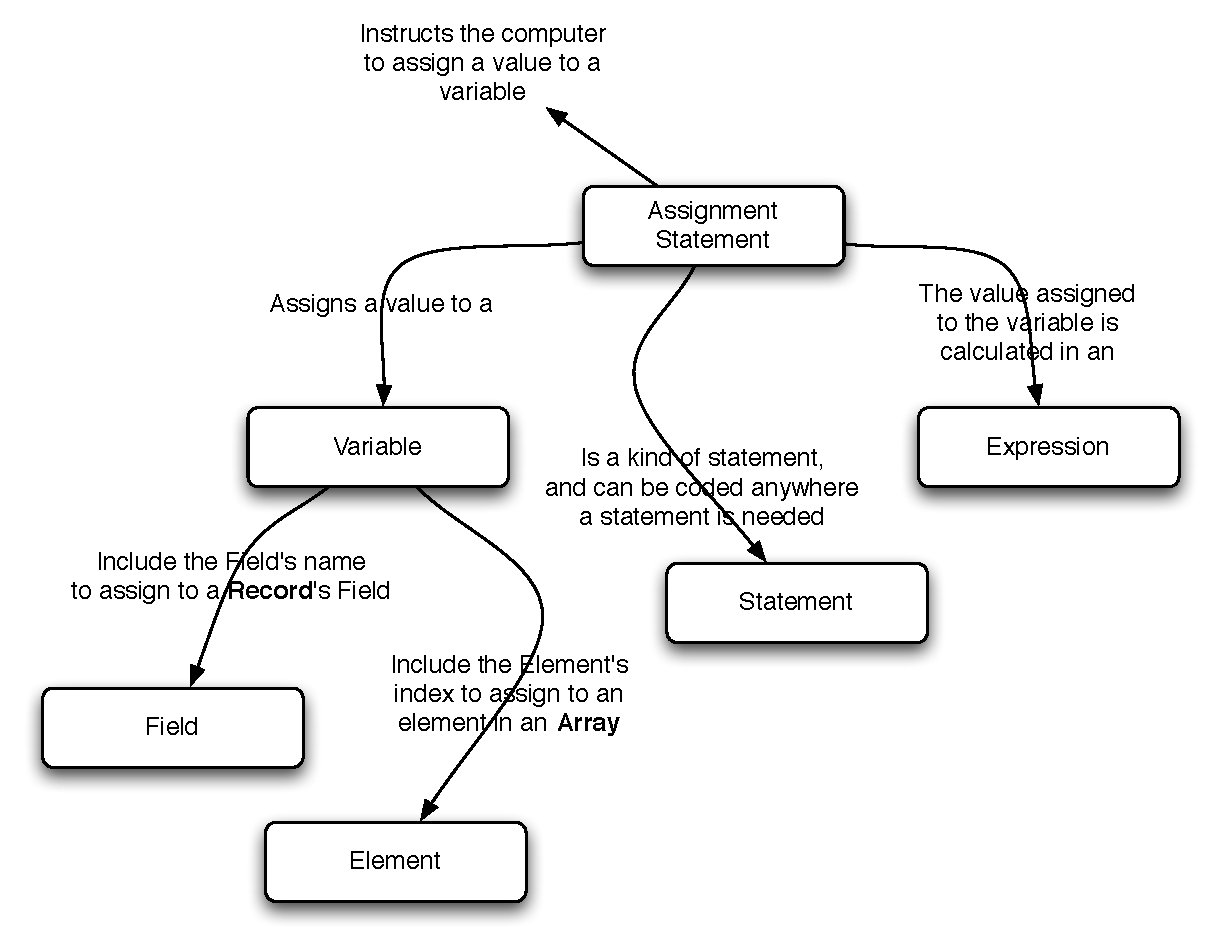
\includegraphics[width=\textwidth]{./topics/type-decl/diagrams/Assignment} 
   \caption{You can assign values to a Record or Union's fields}
   \label{fig:type-decl-assignment}
\end{figure}

\mynote{
\begin{itemize}
  \item The Assignment Statement is an \textbf{action}, you can command the computer to store a value in a variable, array element, record's field, or union's field.
  \item Enumeration values are stored in a single variable, so they work in the same way as shown in \sref{sub:assignment_statement} \nameref{sub:assignment_statement}.
  \item With a record you can assign values to its fields individually, or you can assign it all of the values from another matching record.
  \item A union can have its value set via its fields, or you can copy the value from another matching union.
\end{itemize}
}

\clearpage
\subsubsection{Record Assignment} % (fold)
\label{ssub:record_assignment}

The assignment statement can be used to assign a value to a record's fields, or to copy an existing record's values.

\begin{figure}[h]
   \centering
   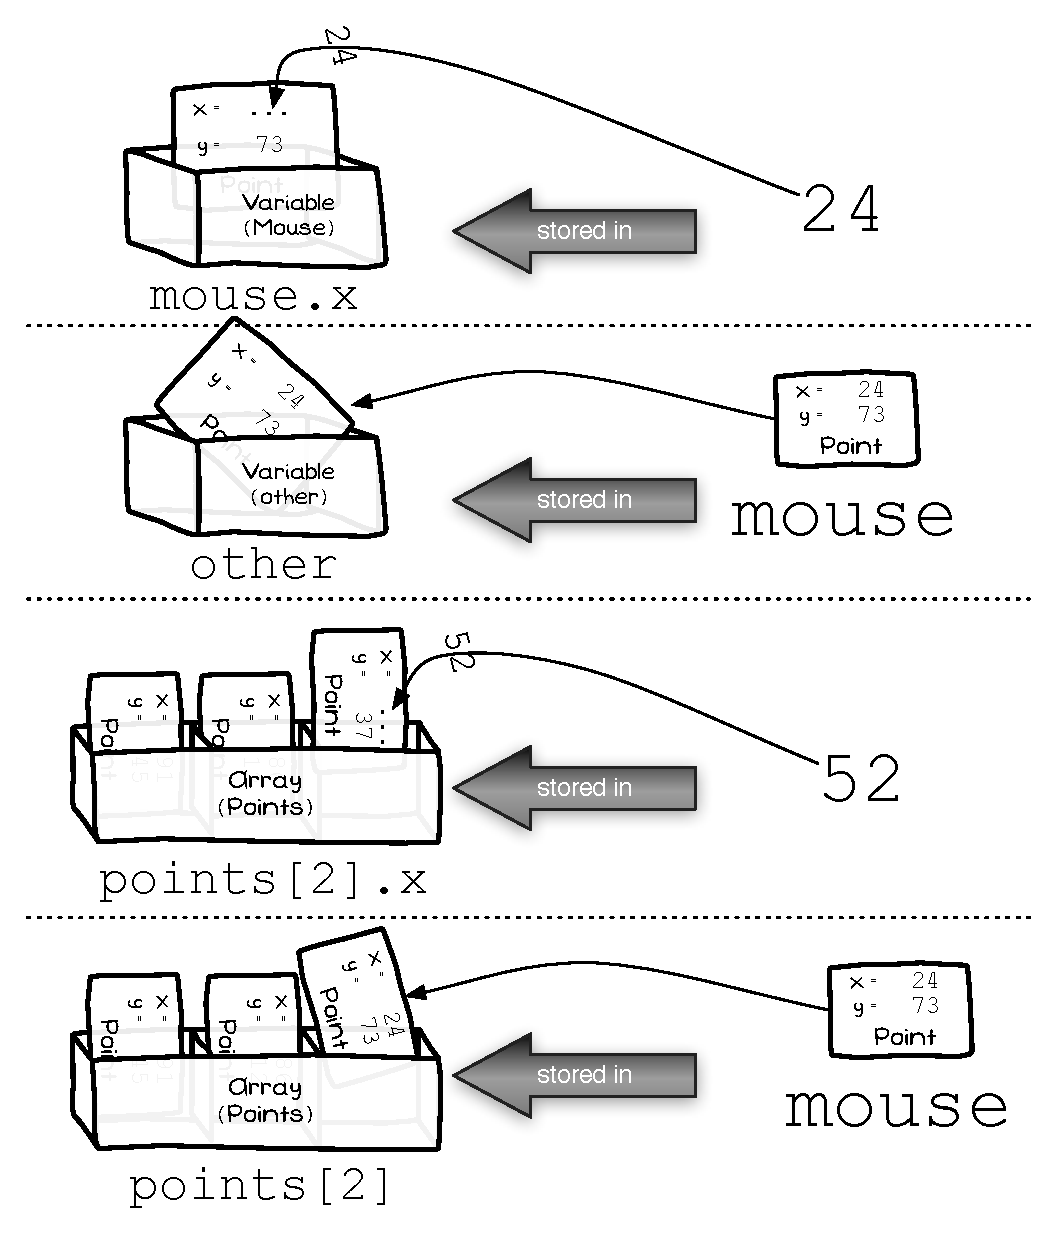
\includegraphics[width=0.8\textwidth]{./topics/type-decl/diagrams/RecordAssign} 
   \caption{You can assign an individual field or the entire record in one assignment statement}
   \label{fig:record-assign}
\end{figure}

\mynote{
\begin{itemize}
  \item The four examples from \ref{fig:record-assign} show the following:
  \begin{enumerate}
    \item You can assign a value to a field of a record. In this case 24 is assigned to \texttt{mouse.x}.
    \item A \texttt{Point} expression can be assigned to a \texttt{Point} variable. This copies the entire record into the Variable.
    \item It doesn't matter if the record is in an array, you can still assign a value to an record's fields.
    \item You can also assign an entire record into an element of an array.
  \end{enumerate}
  \item If the language allows arrays to be copied then you can also copy an entire array of records to a destination.
\end{itemize}
}

% subsubsection record_assignment (end)

\clearpage
\subsubsection{Union Assignment} % (fold)
\label{ssub:union_assignment}

The \nameref{ssub:union} is similar to a Record in that you can assign values to a union via its fields or by copying another union value into the variable or array element. The difference with the Union is that it has only a single value, with the different fields giving you different interpretations of that data.

\begin{figure}[h]
   \centering
   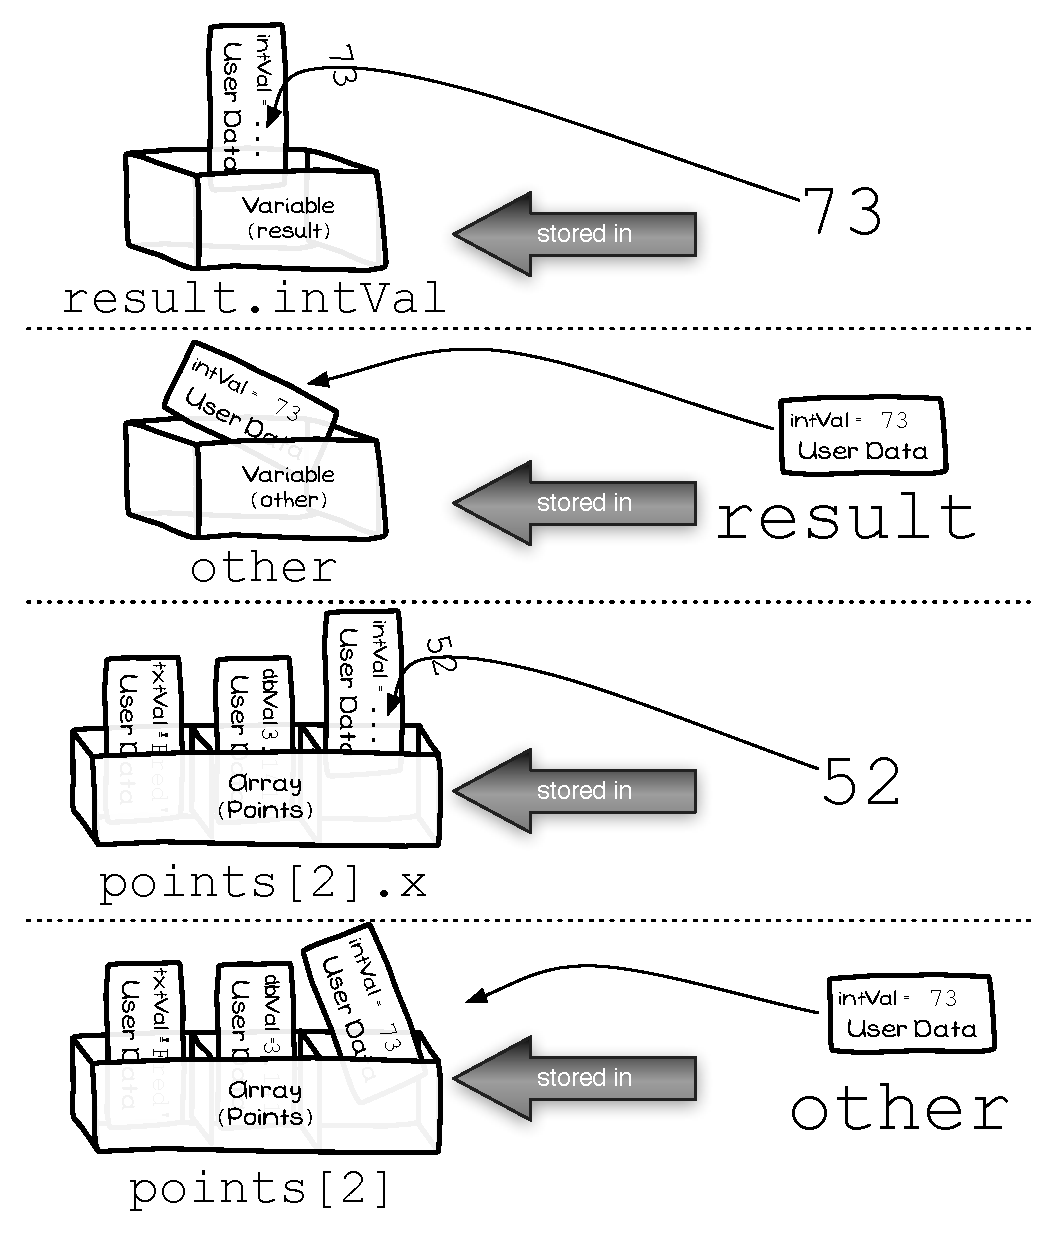
\includegraphics[width=0.8\textwidth]{./topics/type-decl/diagrams/UnionAssign} 
   \caption{You can assign an individual field or the entire union in one assignment statement}
   \label{fig:union-assign}
\end{figure}

\mynote{
\begin{itemize}
  \item The four examples from \ref{fig:union-assign} show the following:
  \begin{enumerate}
    \item You can assign a value to the fields of a Union. This overrides any value currently stored in the Variable.
    \item It is possible to copy an entire Union value in the assignment.
    \item This works in the same way with arrays, you can write a value to an Union.
    \item You can also copy an existing union value into an element.
  \end{enumerate}
  \item When accessing the data in a Union you are responsible for ensuring you read back the value you stored as it does not remember the kind of value you stored in the union.
\end{itemize}
}


% subsubsection union_assignment (end)

% subsection assignment_statement_with_fields_and_elements_ (end)
\clearpage
\subsection{Expression (with custom types)} % (fold)
\label{sub:expression_with_custom_types}

The types you define allow you to specify how data values can be formatted, allowing you to declare variables that contain data in this new format. You can then read data back from your variables in expressions.

\begin{figure}[h]
   \centering
   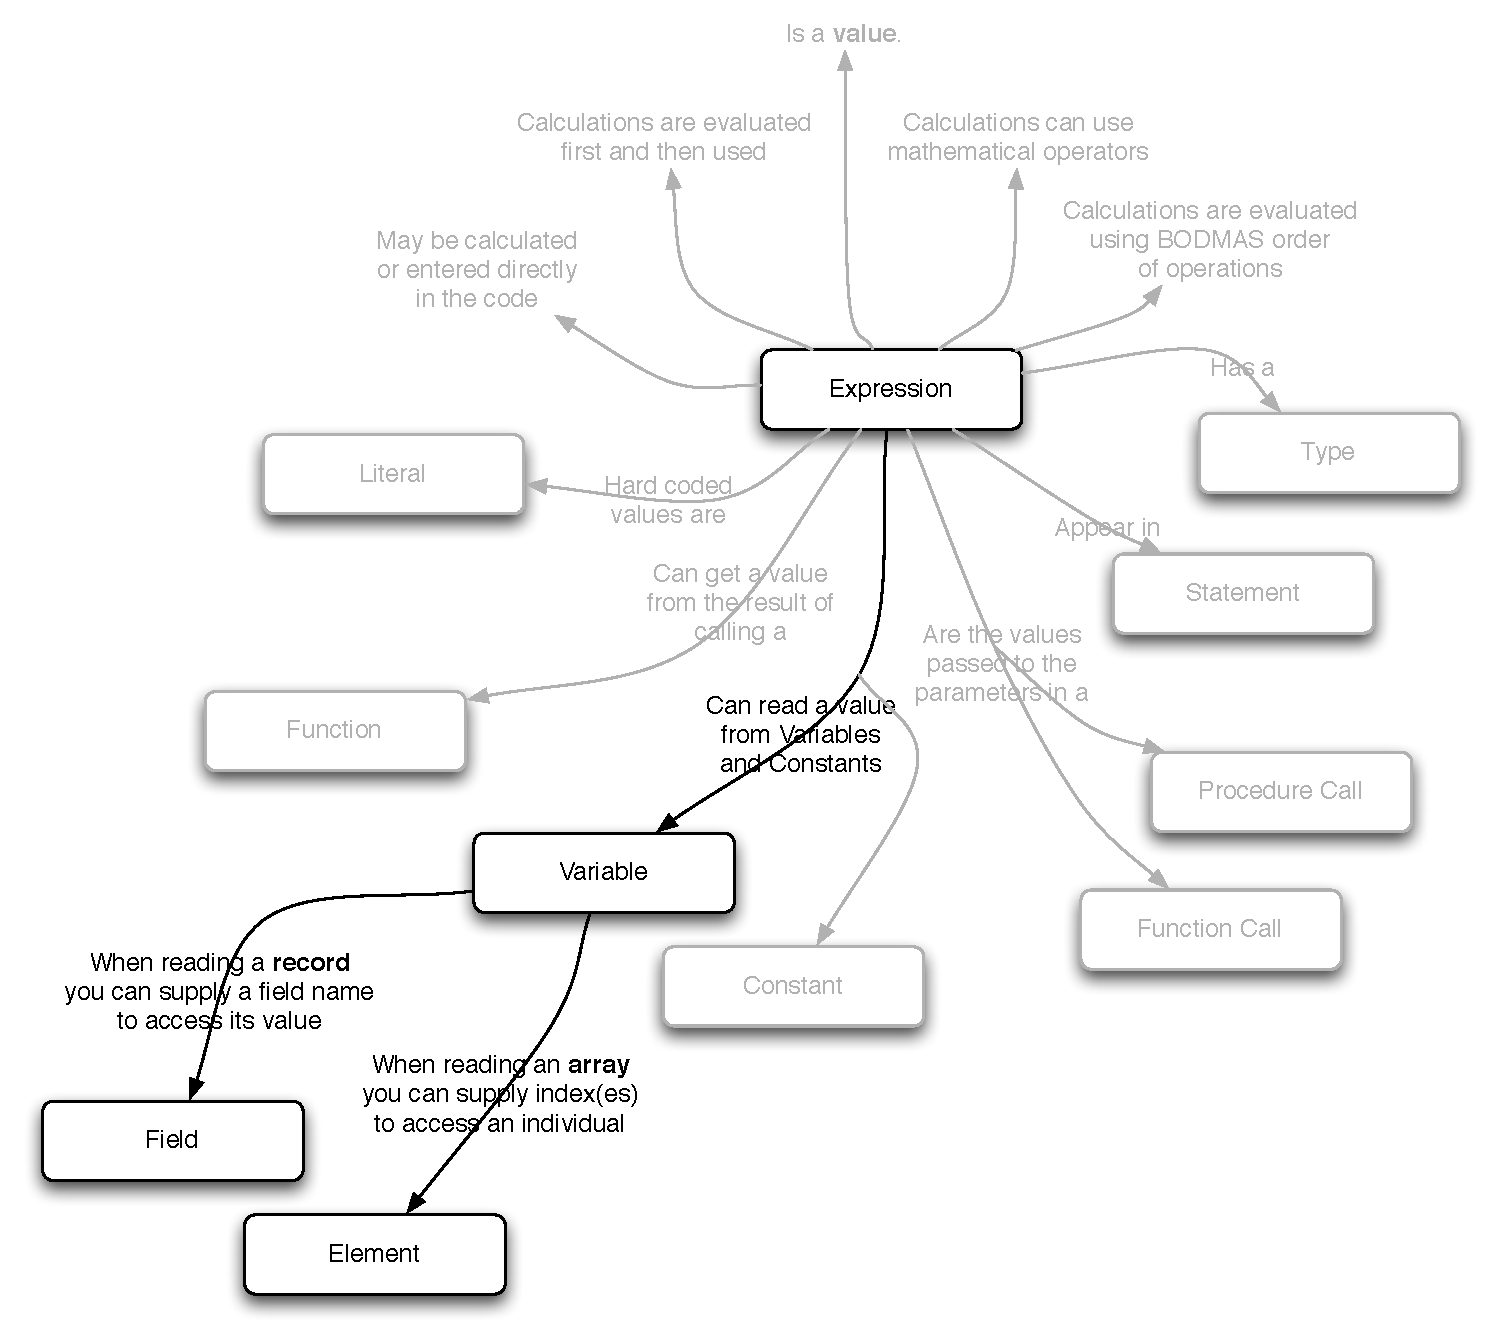
\includegraphics[width=\textwidth]{./topics/type-decl/diagrams/Expression} 
   \caption{An expression can read the value of a record's field, a union's field, and from an enumeration}
   \label{fig:type-decl-expression}
\end{figure}

\mynote{
\begin{itemize}
  \item Expression is the \textbf{term} given to the code that calculates values within your Statements.
  \item Within an expression you can read the value from\ldots
  \begin{itemize}
    \item a field of a record.
    \item a field of a union.
    \item an enumeration.
  \end{itemize} 
  \item The dot (\texttt{.}) notation is used to indicate which field you want to access from a record or union.
\end{itemize}
}

\clearpage
\subsubsection{Record Expressions} % (fold)
\label{ssub:record_expressions}

A \nameref{ssub:record} is a type that contains a number of fields. When using a record value you can use either an individual fields from the record, or the record in its entirety.

\begin{figure}[h]
   \centering
   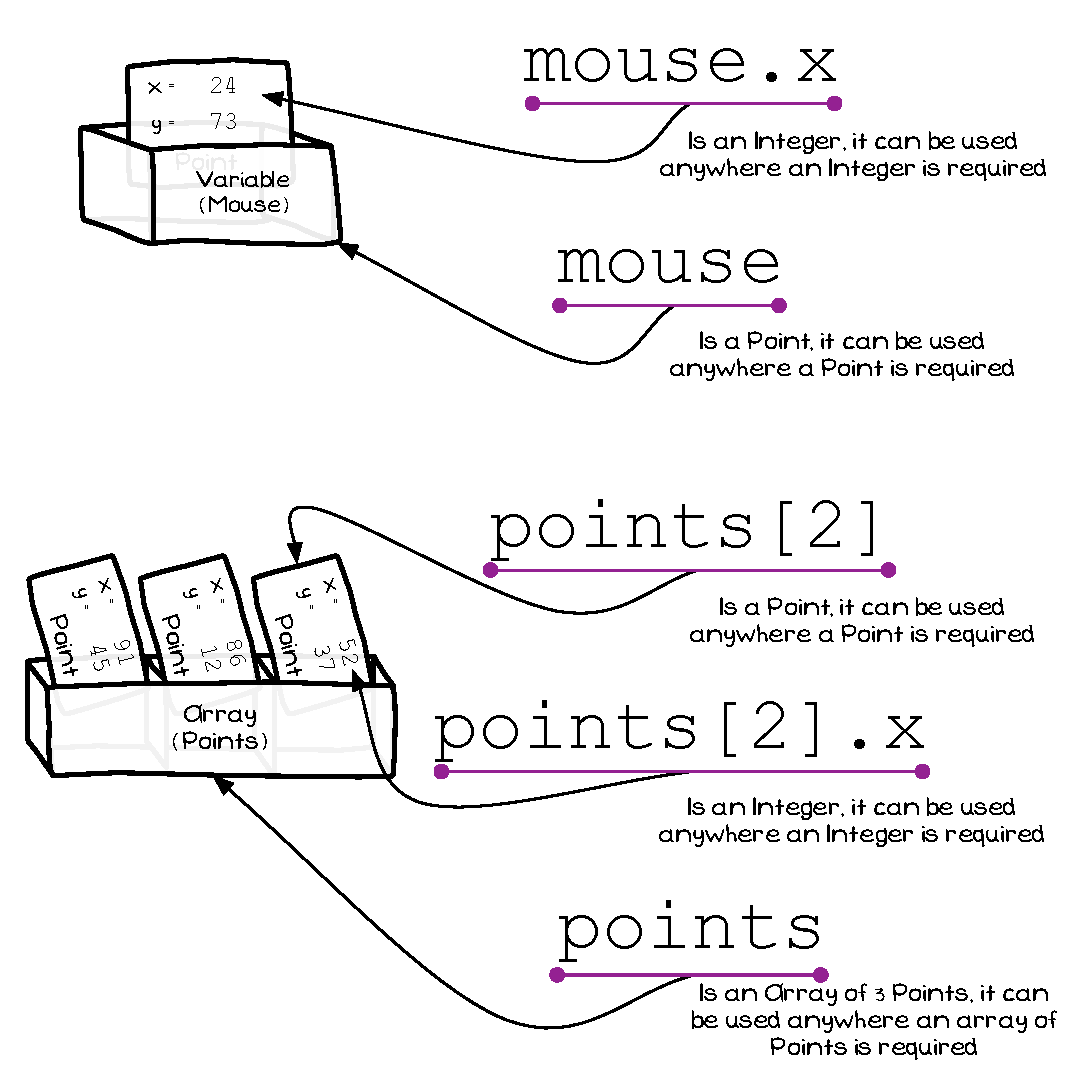
\includegraphics[width=0.8\textwidth]{./topics/type-decl/diagrams/RecordExpr} 
   \caption{A field of a record can be used, or the record can be used in its entirety}
   \label{fig:record-expr}
\end{figure}

\mynote{
\begin{itemize}
  \item \fref{fig:record-expr} shows some examples of expressions on an record variable and array.
  \item The \texttt{Point} record in the illustration has an \texttt{x} field that stores an integer value.
  \item You can access a field of the record from its variable using the dot notation. So \texttt{mouse.x} reads the \texttt{x} value form the record stored in the \texttt{mouse} variable. This value is then an Integer, and can be used anywhere an Integer is allowed. For example, you could have this in an equation where the value was subsequently stored in an Integer variable or passed to an integer parameter.
  \item You can access the entire record using just \texttt{mouse}. This expression has the \texttt{Point} type. It can be used anywhere a Point can be used. For example, it could be stored in another \texttt{Point} variable, or passed to a \texttt{Point} parameter.
  \item In an array of records, each element has the records type. In \fref{fig:record-expr} the \texttt{points} array is storing 3 \texttt{Point} values. This means the \texttt{points} is an expression to access the entire array, \texttt{points[2]} accesses the $3^{rd}$ element and therefore has a \texttt{Point} type, and \texttt{points[2].x} accessed the \texttt{x} value of the $3^{rd}$ element of the \texttt{points} array.
\end{itemize}
}

% subsubsection record_expressions (end)

\subsubsection{Union Expressions} % (fold)
\label{ssub:union_expressions}

A \nameref{ssub:union} has multiple fields that all give access to the same piece of memory. In effect, the union stores only \emph{one} of the values from its available fields. This allows you to create a type that can be used to store one of a selection of available values.

\begin{figure}[h]
   \centering
   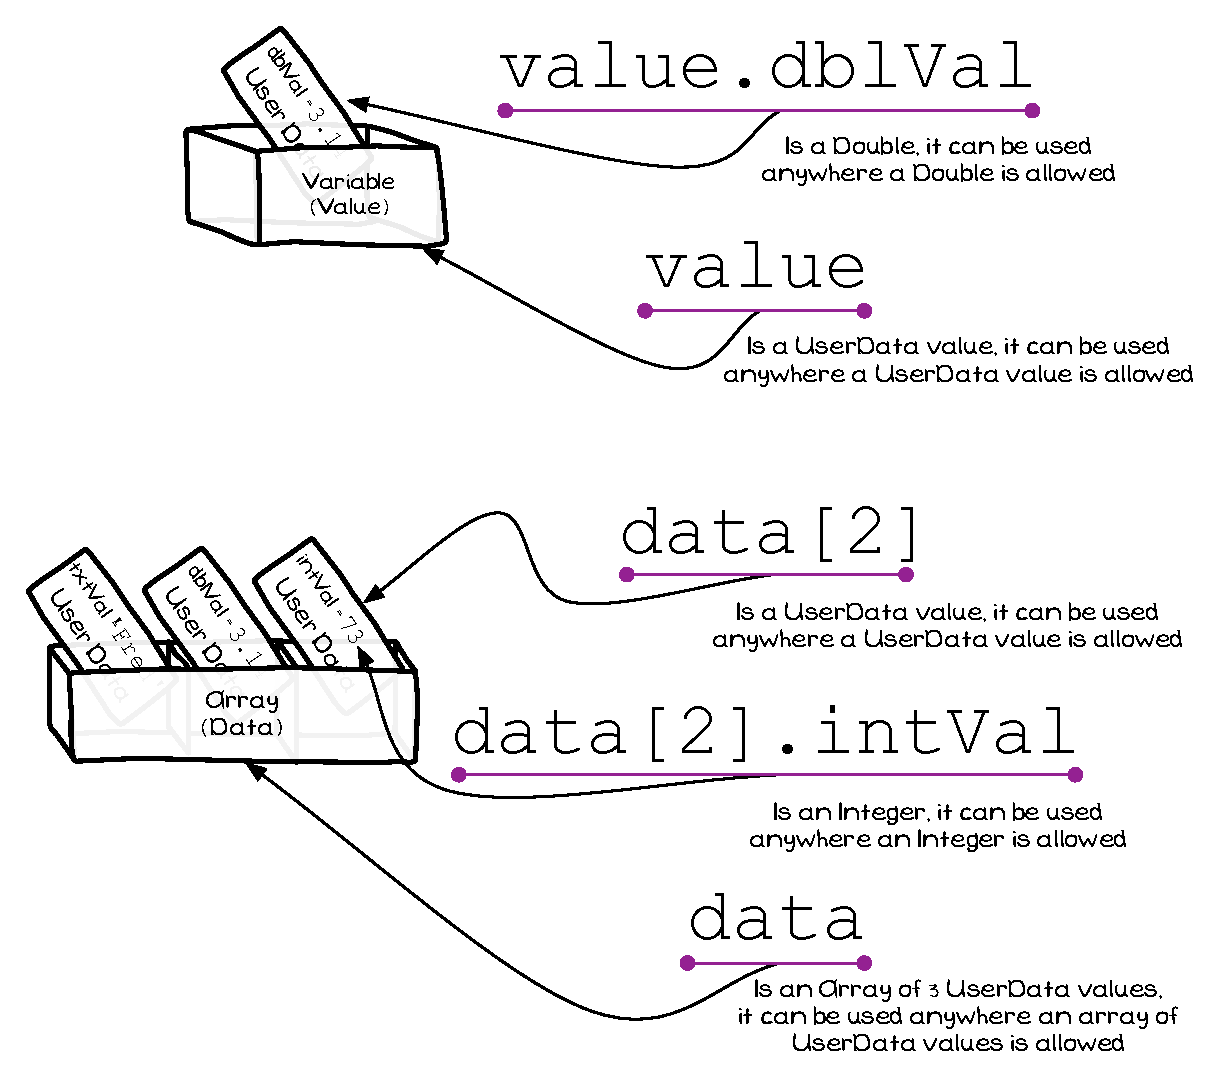
\includegraphics[width=0.87\textwidth]{./topics/type-decl/diagrams/UnionExpr} 
   \caption{A field of a union can be used, or the union can be used in its entirety}
   \label{fig:union-expr}
\end{figure}

\mynote{
\begin{itemize}
  \item A Union is very similar to a Record, the only difference is that the union only stores one of the field values.
  \item \fref{fig:union-expr} shows an example of a union variable and array.
  \item The expression \texttt{value} gives access to the union stored in the variable. This has a \texttt{UserData} type an can be used anywhere a \texttt{UserData} value can be accepted.
  \item The expression \texttt{value.dblVal} is a \texttt{Double} value, and can be used anywhere a \texttt{Double} is allowed.
  \item Accessing a union value from an array is similar to accessing a record value. In \fref{fig:union-expr} you can access the array in its entirety using \texttt{data}, you can access the first \texttt{UserData} value using \texttt{data[0]}, and you can access its text value using \texttt{data[0].txtVal}.
  \item When accessing the data in a Union you are responsible for ensuring you read it using the correct field. For example, it is possible to read the data stored in \texttt{value} using \texttt{value.intVal}. This will not cause any errors during compiling or running, but the value read will be the Integer interpretation of the Double value stored in the variable.
\end{itemize}
}

% subsubsection union_expressions (end)

\clearpage
\subsubsection{Enumeration Expression} % (fold)
\label{ssub:enumeration_expression}

The \nameref{ssub:enum} is the simplest of the custom types to make use of. It defines a list of available options for values of this type. This means that enumerations are just like standard values.

\begin{figure}[h]
   \centering
   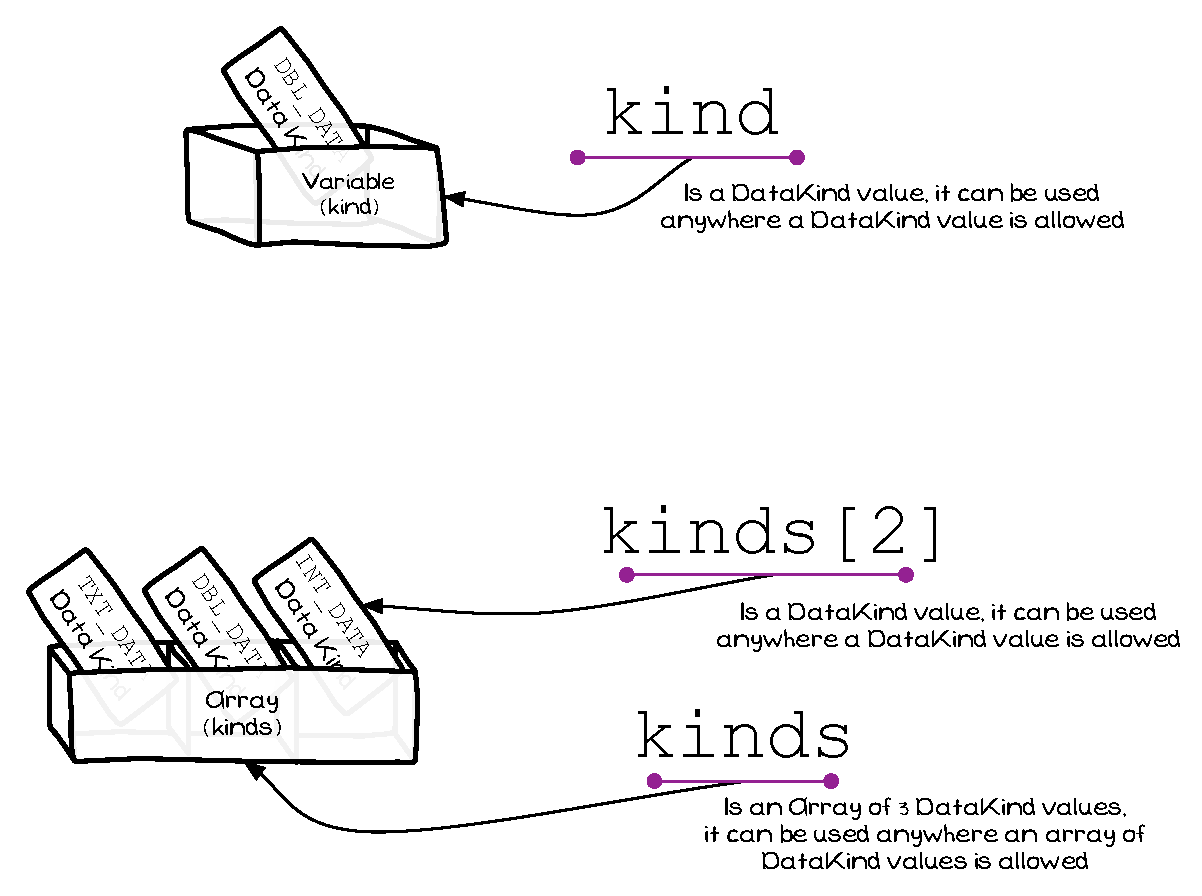
\includegraphics[width=0.87\textwidth]{./topics/type-decl/diagrams/EnumExpr} 
   \caption{You interact with an Enumeration just like other simple data types (Integers, and Doubles for example)}
   \label{fig:enum-expr}
\end{figure}

\mynote{
\begin{itemize}
  \item Accessing an value of an Enumeration type is just like accessing an Integer or Double value.
  \item In \fref{fig:union-expr} the \texttt{kind} variable is storing a \texttt{Data Kind} value. This value can be read from the variable using the variable's name (its \nameref{sub$1$2$3:identifier}).
  \item The \texttt{kinds} variable is an array of \texttt{Data Kind} values. The expression \texttt{kinds} is an array of \texttt{Data Kind} values and can be used anywhere the array would be accepted. \texttt{kinds[0]} is a \texttt{Data Kind} value and can be used anywhere a \texttt{Data Kind} value can be used.
\end{itemize}
}

% subsubsection enumeration_expression (end)

% subsection expression_with_records_and_arrays_ (end)

% section data_type_concepts (end)

% ======================
% = Using Custom Types =
% ======================
\clearpage
\section{Using Custom Types} % (fold)
\label{sec:using_custom_types}

Designing your own data types means that your code can work with more meaningful values. You can design the data that is stored in the program so that it is organised in ways that will help make the processing simpler.

\subsection{Designing Small DB} % (fold)
\label{sub:designing_small_db}

\tref{tbl:small-db-prog} contains a description of the Small DB program that will be explored in this chapter. This is a small program that will read, store, and output values entered by the user.

\begin{table}[h]
\centering
\begin{tabular}{l|p{10cm}}
  \hline
  \multicolumn{2}{c}{\textbf{Program Description}} \\
  \hline
  \textbf{Name} & \emph{Small DB} \\
  \\
  \textbf{Description} & Reads text (up to 7 characters), integer, and double values from the user, storing them within the program and then outputting their values to the Terminal along with the type being stored in the program. Each value will be stored in a row with a unique identifier that will be assigned by the system. The first value will be assigned the id 0, the second will be assigned the id 1, and so on.\\
  \hline
\end{tabular}
\caption{Description of the Small DB program.}
\label{tbl:small-db-prog}
\end{table}

As before, the process to design and implement this program will follow a number of steps:
\begin{enumerate}
  \item Understand the problem, and get some ideas on the tasks that need to be performed.
  \item Choose the artefacts we will create and use
  \item Design the control flow for the procedural\footnote{The Program, and any Functions and Procedures.} artefacts
  \item Map these artefacts to code
  \item Compile and run the program
\end{enumerate}

% subsection designing_small_db (end)

\subsection{Understanding Small DB} % (fold)
\label{sub:understanding_small_db}

This program does not perform any complex functionality, so it does not require much analysis to understand the tasks that need to be performed.

Data identified:
\begin{itemize}
  \item \textbf{Row}: has a unique identifier, and a value.
  \item \textbf{Column Value}: each value in a row is either an integer, a double, or a text value.
\end{itemize}

Tasks to be performed:
\begin{itemize}
  \item \textbf{Read Row}: The program needs to be able to read a row from the user.
  \item \textbf{Print Row}: After reading the value the program need to output the value to the Terminal.
\end{itemize}

% subsection understanding_small_db (end)
\clearpage
\subsection{Choosing Artefacts for Small DB} % (fold)
\label{sub:choosing_artefacts_for_small_db}

The process of choosing the artefacts for a program involves determining both the structure of the data, as well as the structure of the functions and procedures. In many cases the structure of the data is more important than the structure of the functionality, as getting the data right will make the processing easier. Therefore, the first task is to consider how the data can be structured.

The three main tools that you have for designing the structure of the data in your program are \textbf{records}, \textbf{unions}, and \textbf{enumerations}. A record allows you to create a composite data type that is made up of a number of fields. The union allows you to create a type that stores one kind of data, or another. Finally the enumeration allows you to create a list of available options.

\subsubsection{Looking for records in Small DB} % (fold)
\label{ssub:looking_for_records_in_small_db}

The most common of these is the \textbf{record}, a \textbf{struct} in C. This type allows you to create a single composite value that is composed of a number of related field values. This can be used to model the \emph{entities} in your program. When designing with records you think about the things you want to model, and the data associated with these things.

In the case of the Small DB program there appears to be one kind of record: the \texttt{row}. The program needs to store \textbf{row} values, where each row has a unique id (an integer), and a data value. These two values \emph{together} make up a row.

This data type will also work nicely with the planned functionality for the program. The code needs to be able to read and print \texttt{row} values. This means that this code can accept/return \texttt{row} values. The \texttt{Print Row} procedure will take in a \texttt{row} parameter, and print out its details to the \texttt{Terminal}. The \texttt{Read Row} function can read values from the user and return a \texttt{row} value to the caller.

% subsubsection looking_for_records_in_small_db (end)

\subsubsection{Looking for unions in Small DB} % (fold)
\label{ssub:looking_for_unions_in_small_db}

The \textbf{union}\footnote{\textbf{Variant record} in Pascal} is going to be less common than records, but they can offer some useful flexibility when designing your code. The union gives you the ability to have a type that stores one of a selection of types. If your program requires the ability to store different types at the one location then a union is a useful way of modelling this.

Reading the description of the Small DB program there does appear to be the need for a union. Each \texttt{row} needs to be able to store \emph{either} a Integer, a Double, or a text value. Using a union it will be possible to create a type to model this. This can be called the \texttt{Column Value} type, and will be the union of these three values.

The great thing about a union is that it stores only one value, the one that you assign to it. This means that it takes only the size needed to store the largest kind of value. In our case the \texttt{Column Value} will need space to store an Integer (4 bytes), a Double (8 bytes), or 7 Characters (8 bytes, 7 + 1 overhead). This will only need \textbf{8 bytes} of space, as at any one time it can only have one of these values. 

% subsubsection looking_for_unions_in_small_db (end)

\subsubsection{Looking for enumerations in Small DB} % (fold)
\label{ssub:looking_for_enumerations_in_small_db}

The last type to look for is the enumeration. This can be used to code a list of available options. Reading through the description of the program there is no really obvious list of options, but on further analysis there may be.

Remember that the Union does not know which value you stored in it. So you would be able to store a value in a Row, but then you would not know which value to read back from the union. This is where an enumeration can come in handy. You can create an enumeration that gives options for each of the kinds of values that the union can store. In this case the options can be \texttt{INT\_VAL}, \texttt{DBL\_VAL}, and \texttt{TXT\_VAL}, and can be called \texttt{Data Kind}.

The \texttt{Data Kind} enumeration allows you to declare variables that will have one of the available options as its value. This value will need to be stored for each \texttt{Row} in the program, so a field needs to be added to the \texttt{Row} type. This \texttt{kind} field can then store a marker that indicates the kind if value that is stored in the record.

This is a common pattern you will find for working with unions. It is called a \textbf{tagged union}. The enumeration value is the \textbf{tag} and stores an indicator of the kind of value stored in the union. This is the model behind the implementation of unions in Pascal, but must be manually coded in C.

% subsubsection looking_for_enumerations_in_small_db (end)

\subsubsection{Overall data design} % (fold)
\label{ssub:overall_data_design}

\tref{tbl:dd-small-db} shows the structures chosen for the data Small DB program. These provide the data model that will be used by the code to implement the program's logic. Having planned out the structure for the data of this program, the next step will be to design its logic.

\begin{table}[htbp]
  \centering
  \begin{tabular}{|l|l|l|}
    \hline
    \textbf{Data} & \multicolumn{2}{c|}{\textbf{Details}}  \\ 
    \hline
    \multicolumn{3}{c}{} \\
    \hline
    \textbf{\texttt{Row}} & \multicolumn{2}{l|}{A \textbf{record/struct} with the following fields:}  \\
    \hline
    & \texttt{id} & An \textbf{Integer} value that stores the unique id. \\
    \hline
    & \texttt{kind} & A \textbf{Data Kind} value indicating the type of data being stored in this record. \\
    \hline
    & \texttt{data} & Stores \textbf{Column Value} data containing the actual data. \\ 
    \hline
    \multicolumn{3}{c}{} \\
    \hline
    \textbf{\texttt{Data Kind}} & \multicolumn{2}{l|}{A \textbf{enumeration} with the following options:}\\
    \hline
    & \texttt{INT\_VAL} & Indicates the row is storing an Integer value. \\
    \hline
    & \texttt{DBL\_VAL} & Indicates that the row is storing a Double value. \\
    \hline
    &  \texttt{TXT\_VAL} & Indicates that the row is storing a text value. \\
    \hline
    \multicolumn{3}{c}{} \\
    \hline
    \textbf{\texttt{Column Value}} & \multicolumn{2}{l|}{A \textbf{union} that stores one of the following:}\\
    \hline
    & \texttt{Int Val} & An Integer value. \\
    \hline 
    & \texttt{Dbl Val} & A Double value. \\
    \hline
    & \texttt{Txt Val} & A text value, with up to seven characters. \\
    \hline
  \end{tabular}
  \caption{Data Dictionary for Small DB}
  \label{tbl:dd-small-db}
\end{table}

% subsubsection overall_data_design (end)

\subsubsection{Reading a Row} % (fold)
\label{ssub:reading_a_row}

The first piece of functionality to implement can be the \texttt{Read Row} function. This function will be responsible for reading a value from the user, and determining if that value is an integer, double, or string and then storing it in the row with the correct tag value.

To implement this will require the ability to check if the value in a string is an integer or a double. These two tasks can be coded into functions \texttt{Is Integer} and \texttt{Is Double}. Other than this the remaining code just needs to copy values into the fields of the \texttt{Row} that will be returned.

\texttt{Read Row} will need to accept a single parameter, \texttt{Next Id}. This will be the value assigned to the \texttt{id} field of the \texttt{Row}, and will be passed in as this data will be managed elsewhere. At the end of the function, \texttt{Read Row} will return a single \texttt{Row} value. As this is a \textbf{record}, it will contain \texttt{id}, \texttt{kind}, and \texttt{data} values.

\begin{figure}[p]
   \centering
   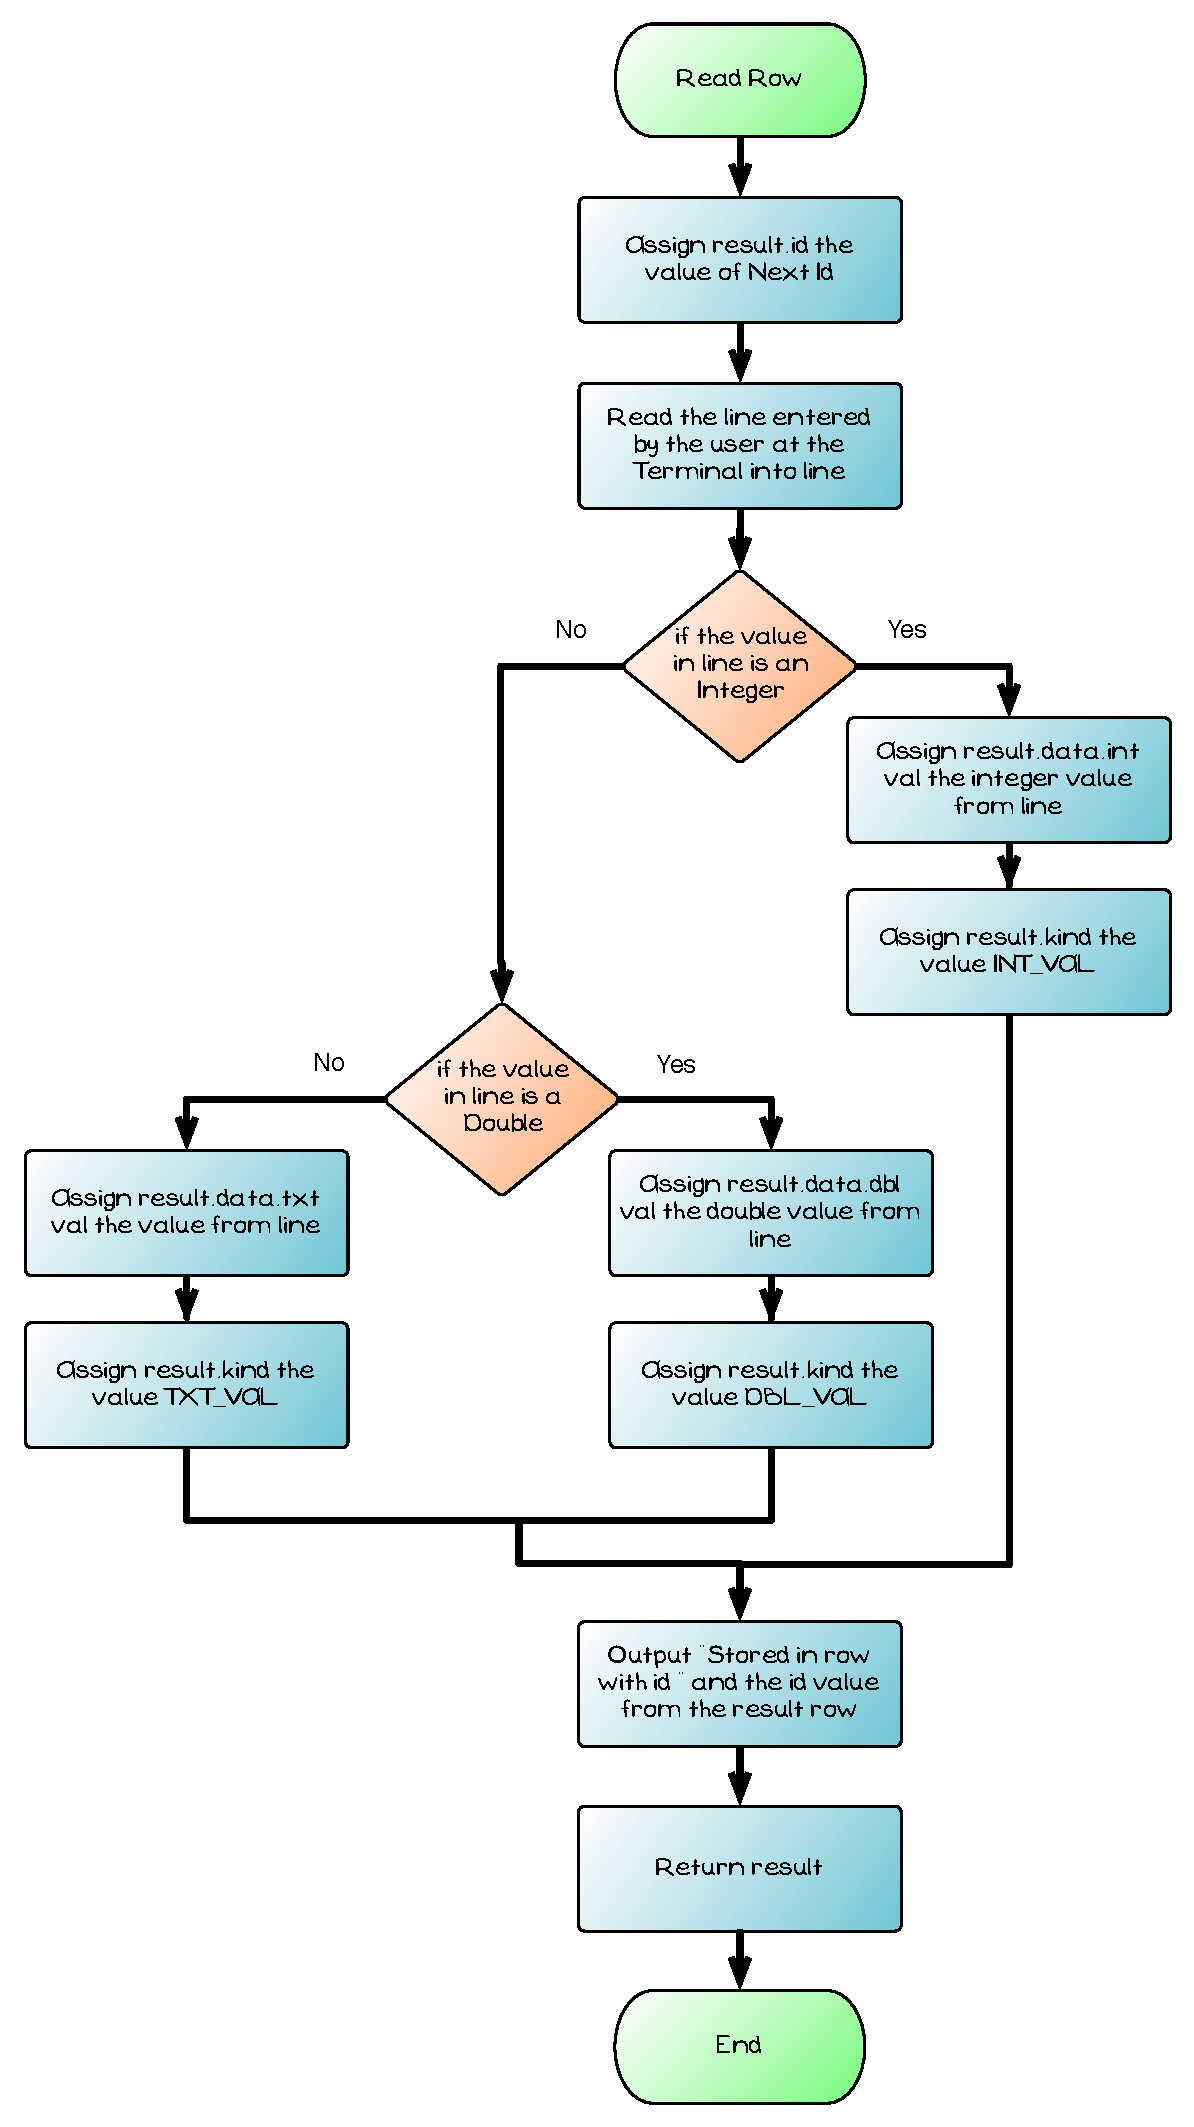
\includegraphics[width=0.80\textwidth]{./topics/type-decl/diagrams/ReadRowFlow} 
   \caption{Flowchart for \texttt{Read Row}}
   \label{fig:read-row-flow}
\end{figure}

\fref{fig:read-row-flow} shows the flowchart for the steps in the \texttt{Read Row} function. Notice that all three fields of the \texttt{Row} are assigned values. The \texttt{id} is assigned in the first statement, whereas the \texttt{data} and \texttt{kind} fields are assigned values in the branches of the if statements. All of this data is then returned when the result value is returned.

The \textbf{union} is being used when the \texttt{data} field is assigned a value. When the \emph{integer} branch is taken the union is assigned a value via its \texttt{int val} field. When the \emph{double} branch is taken the union is assigned a value via its \texttt{dbl val} field. When neither of these branches is taken, the \emph{text} value is assigned to the union via its \texttt{txt val} field.

Finally, one of the options from the \textbf{enumeration} is stored in the \texttt{kind} field of the record alongside the union's value. This means that the \texttt{INT\_VAL} value is stored in the \texttt{kind} field when the \emph{integer} branch is taken, and the \texttt{DBL\_VAL} value is stored when the \emph{double} branch is taken, and the \texttt{TXT\_VAL} value is stored when the \emph{text} path is taken.

\fref{fig:read-row-data} shows three examples of the kinds of values that could be the \texttt{result} of this function when it returns. In each case there are three field values in the row. These are defined in the \texttt{Row} record, and include the \texttt{id}, the \texttt{kind}, and the \texttt{data}.

\begin{figure}[htbp]
   \centering
   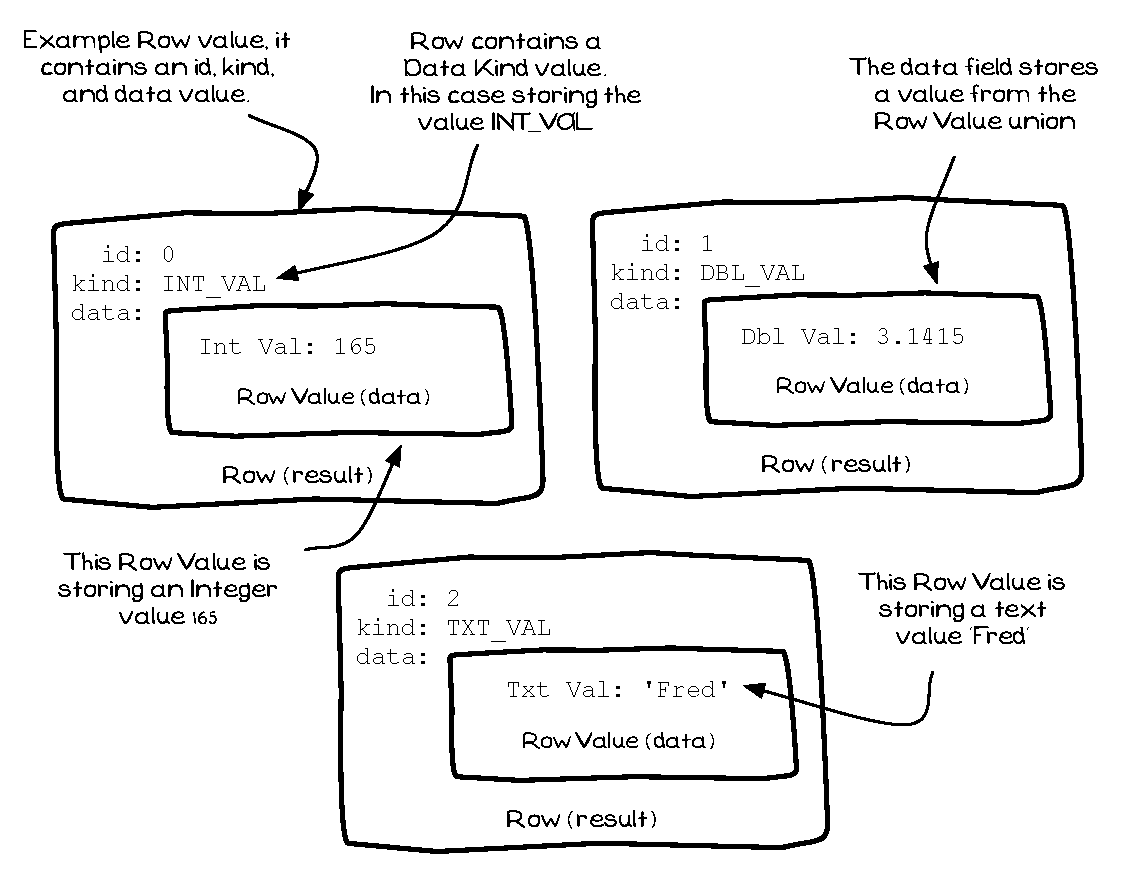
\includegraphics[width=0.8\textwidth]{./topics/type-decl/diagrams/RowDataRead} 
   \caption{Examples of data that could be read into a \texttt{Row} value in \texttt{Read Row}}
   \label{fig:read-row-data}
\end{figure}

% subsubsection reading_a_row (end)
\clearpage
\subsubsection{Printing a Row} % (fold)
\label{ssub:printing_a_row}

Having read data into a \texttt{Row} it is now possible to output that to the Terminal. The steps required to do this can be coded into a \texttt{Print Row} procedure. The required steps are shown in the flowchart in \fref{fig:print-row-flow}.

The \texttt{Print Row} procedure will take a single \texttt{Row} parameter. This parameter will contain the data related of the row that is to be output to the Terminal. The procedure will output the \texttt{id} value and the \texttt{data} values from the \texttt{Row}, using the \texttt{kind} value to determine which field to access from the \texttt{Column Value} union.

The \texttt{row}'s \texttt{id} can be output straight away as it is an Integer value. The actual data that needs to be output depends on the kind of value that is stored in the \texttt{Row}. A \nameref{sub:case_statement} can be used to select a path based upon the value stored in the row's \texttt{kind} field. The four paths here cater for the three options from the \texttt{Data Kind} enumeration, plus an additional path in case the value in \texttt{To Print}'s \texttt{kind} field does not match\footnote{A enumeration is stored as an Integer value, meaning it is possible to store other values in here.} one of these. This path would indicate a bug in the software, but should be included just to be safe.

\begin{figure}[htbp]
   \centering
   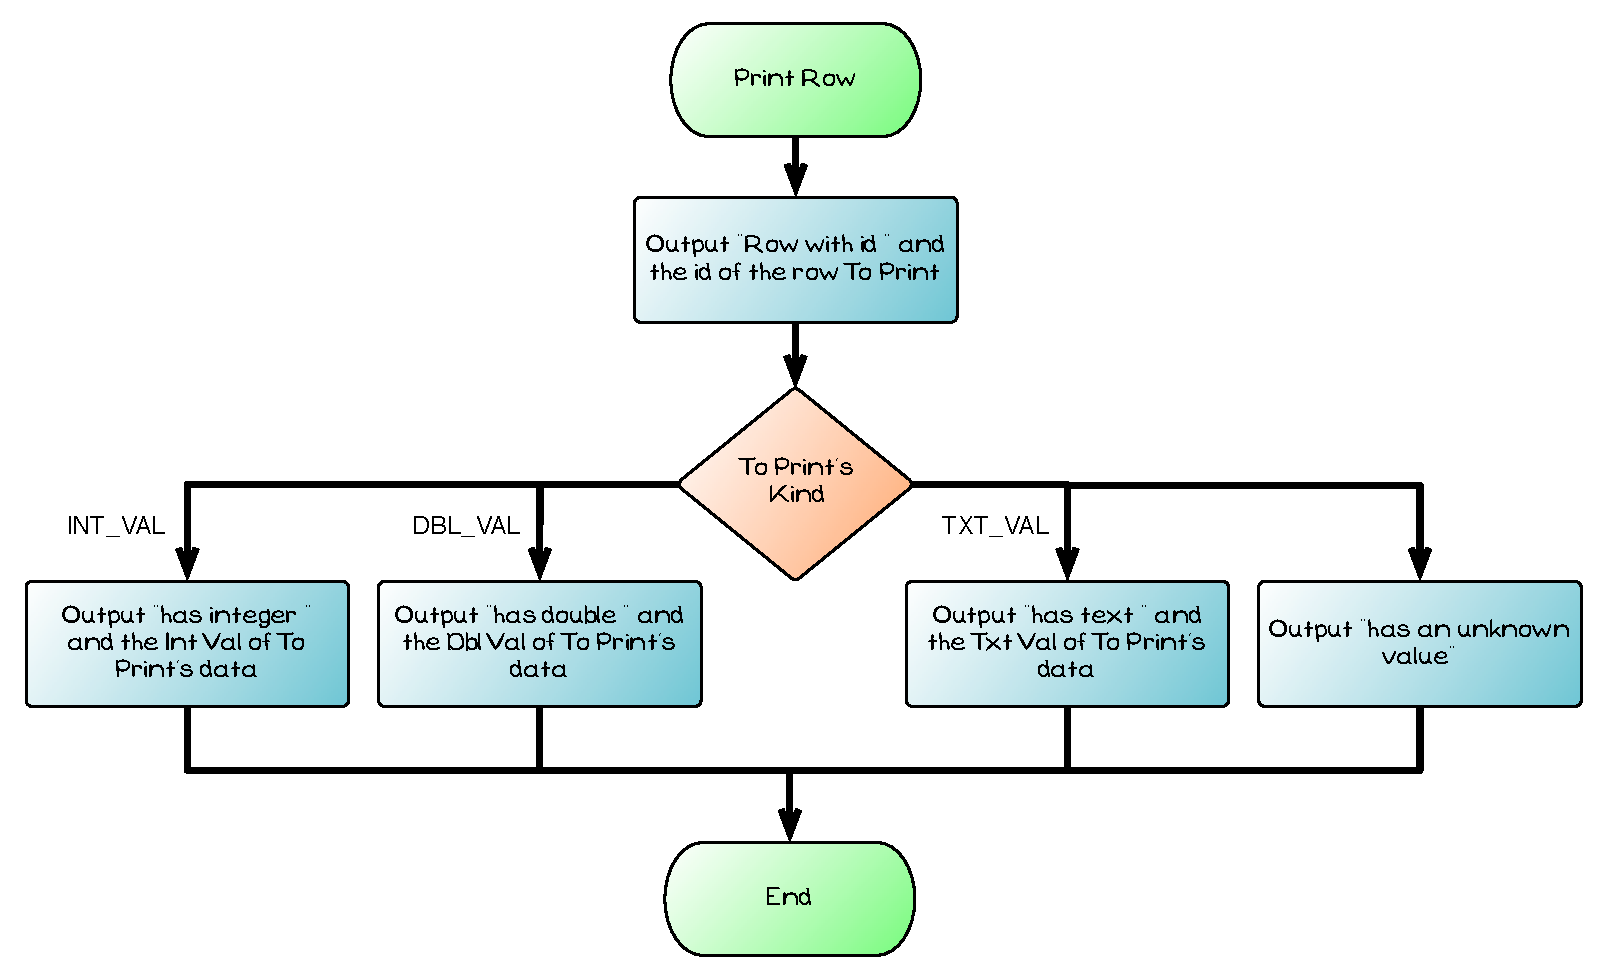
\includegraphics[width=\textwidth]{./topics/type-decl/diagrams/PrintRowFlow} 
   \caption{Flowchart of the steps needed to print a \texttt{Row} to the Terminal}
   \label{fig:print-row-flow}
\end{figure}

% subsubsection printing_a_row (end)
\clearpage
\subsubsection{Overview of Small DB's design} % (fold)
\label{ssub:overview_of_small_db_s_design}

\fref{fig:small-db-struct} shows the structure chart for the design of the Small DB program. The functionality is split between the \texttt{Read Row} function and the \texttt{Print Row} procedure, with \texttt{Is Integer} and \texttt{Is Double} providing useful utility functions to test the data read from the user.

\begin{figure}[htbp]
   \centering
   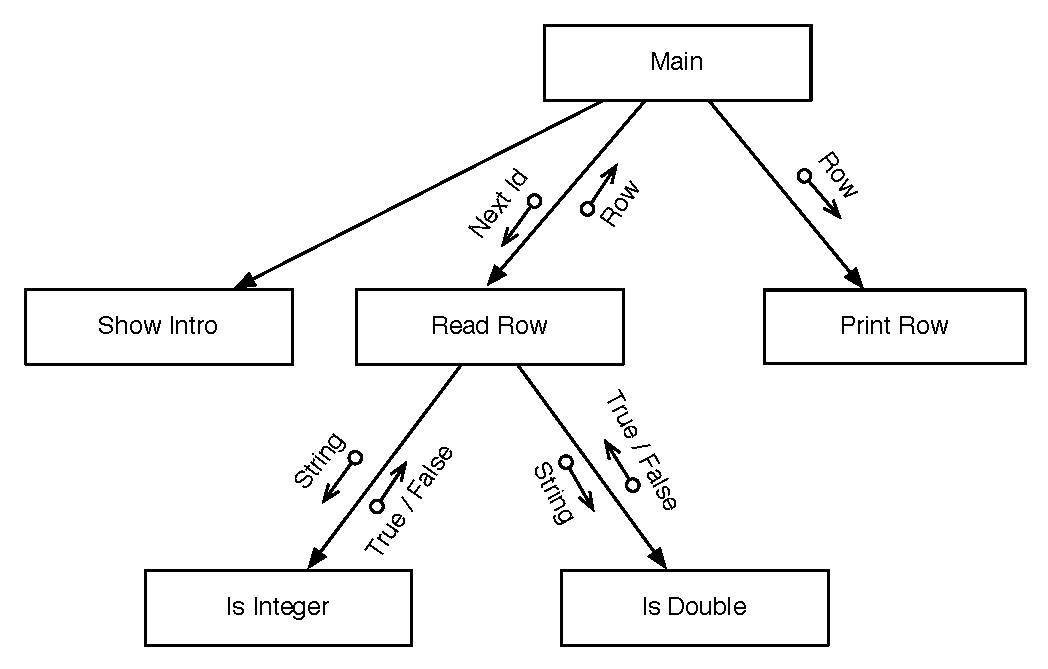
\includegraphics[width=0.85\textwidth]{./topics/type-decl/diagrams/SmallDBStruct} 
   \caption{Structure chart showing the overview of the Small DB program}
   \label{fig:small-db-struct}
\end{figure}

The \texttt{Main} procedure will be responsible for storing the data read from the user in an \nameref{sub:array} of \texttt{Row} values. The logic in \texttt{Main} will then loop over this array once to read in a value \emph{for each} element of the array, using \texttt{Read Row} to get this value. \texttt{Main} with then loop over the array a second time, this time calling \texttt{Print Row} \emph{for each} element in the array. This will allow \texttt{Main} to read in, and then print out, all of the rows.

A \texttt{Show Intro} procedure has also been added to this design to house the code to show the startup message to the user. This moves this code out of the \texttt{main} procedure allowing it to focus on coordinating the tasks involved in working with the array of \texttt{Row} values.

% subsubsection overview_of_small_db_s_design (end)
% subsubsection choosing_artefacts_for_small_db (end)

\subsection{Writing the Code for Small DB} % (fold)
\label{sub:writing_the_code_for_small_db}

The flowcharts and Pseudocode shown communicate the logic that needs to be coded into the Functions and Procedures of this Program. The following two sections, \sref{sec:custom_types_in_c} \nameref{sec:custom_types_in_c} and  \sref{sec:custom_types_in_pas} \nameref{sec:custom_types_in_pas}, contain a description of the syntax needed to code your own types in the C and Pascal programming languages. This information can be used to write the code for the Small DB program, and others.

% subsection writing_the_code_for_small_db (end)

\clearpage
\subsection{Compiling and Running Small DB} % (fold)
\label{sub:compiling_and_running_small_db}

Remember to code and run this one small piece after the other. For this you could start by writing the \texttt{Print Row} procedure, and pass it values that you hard code in the program. This will allow you to experiment with storing different values in the fields of the record and union without having to deal with the user input and testing functions. You can test this by checking that the output matches what you expect based on the values in the \texttt{Row}.

Once this is complete the next task would be to work on the \texttt{Read Row} function, and its helpers. These have a bit more logic and will require that you test it more carefully. Think about the kind of test data that you can use to check each of the paths through these functions, and use this to check your code as you progress.

\fref{fig:small-db-using} shows the program in operation.

\begin{figure}[h]
   \centering
   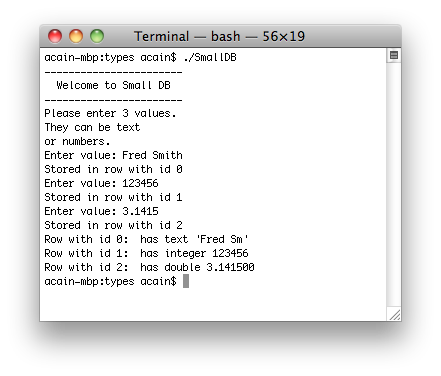
\includegraphics[width=0.9\textwidth]{./topics/type-decl/images/SmallDB} 
   \caption{Small DB run from the Terminal, repeated from \fref{fig:small-db}}
   \label{fig:small-db-using}
\end{figure}


% subsection compiling_and_running_small_db (end)


% section using_custom_types (end)

% =============
% = C Section =
% =============
\clearpage
\def\pageLang{c}
\section{Custom Data Types in C} % (fold)
\label{sec:custom_types_in_c}

\subsection{Implementing Small DB in C} % (fold)
\label{sub:implementing_small_db_in_c}

\sref{sec:using_custom_types} of this Chapter introduced the Small DB program. A partial implementation of this program is shown in \lref{lst:c-small-db}. The type definitions, and code are missing the details needed to store and display double values. This program reads a number of rows of data from the user (determined by the \texttt{DB\_SIZE} constant). Each row stores a single value, being either a double value, an integer value, or a text value.

\straightcode{\ccode{lst:c-small-db}{C code for the Small DB program}{code/c/types/small-db.c}}

\mynote{
\begin{itemize}
  \item \texttt{strtol} is a function from the \texttt{stdlib.h} header. This converts the input to a integer, and updates \texttt{p} to point to the character the conversion got to before ending. Checking that this matches the end of string terminator (\csnipet{'\\0'}) indicates that the input matches the entire string.
  \item \texttt{strtod} is a similar function that converts text to a double. As with \texttt{strtol}, this updates \texttt{p} to refer to the character it got in the conversion. If this refers to the end of the text then the data does contain a double.
  \item The \texttt{trim} function removes spaces from the start and the end of the input, ensuring that numbers with leading or trailing spaces are still detected as numbers.
  \item The type definitions must appear before they are used, as a result they commonly appear at the start of the code after the includes.
  \item \texttt{limits.h} gives access to the constants \texttt{INT\_MAX} and \texttt{INT\_MIN}, these can be used to check if the integer read is in the range of an integer value.
  \item \texttt{errno.h} gives access to the \texttt{errno} global variable that contains an error number when the integer is outside of the range of a long.
  \item The code in \texttt{Read Row} includes code that skips any unwanted input on the current line. This requires two \texttt{scanf} calls: the first reading in any characters other than a newline, and the next reading in the newline. This method of skipping unwanted data in input is safe and works across multiple platforms.
  \item A number of online resources refer to using \texttt{fflush} to skip processing input between reads. This \textbf{should not} be used. The \texttt{fflush} function is used to ensure that output is written to the underlying hardware. The behaviour of this function \textbf{is not defined} for input streams. As a result it will not work as expected on all platforms.
\end{itemize}
}

% subsection implementing_small_db_in_c (end)
\clearpage
\subsection{C Type Declaration} % (fold)
\label{sub:c_type_declaration}

In C you can declare your own record/structure, union, and enumeration types using the \texttt{typedef} declaration. It is also possible to create an alias type declaration, in which you assign a new name to an existing type.

\csyntax{csynt:type-decl-variable-decl}{Type Declarations}{type-decl/type-decl}

\csection{\ccode{clst:test-alias}{Testing the alias declarations in C}{code/c/types/test-alias.c}}

\mynote{
\begin{itemize}
  \item This syntax allows you to declare your own data types.
  \item The following sections contain the details of declaring different kinds of custom types:
  \begin{itemize}
    \item Records/structures are shown in \nameref{sub:c_structure_declaration}.
    \item Enumerations are shown in \nameref{sub:c_enum_declaration}.
    \item Unions are shown in \nameref{sub:c_union_declaration}.
  \end{itemize}
  \item \lref{clst:test-alias} shows how to declare alias types. An alias type give a new name to an existing type. Included in this are examples of the following:
  \begin{itemize}
    \item \texttt{number} is an alias for \texttt{int}.
    \item \texttt{five\_numbers} is an alias for an array of file \texttt{int} values.
    \item \texttt{my\_string} is an alias for a string of 256 characters.
    \item \texttt{c\_string} is an alias for a variable length string.
    \item \texttt{const\_c\_string} is an alias for a read-only c-string.
  \end{itemize}
  \item Notice that these new types can be used to declare variables, arrays, and parameter.
  \item \texttt{grid2} is an array that contains \texttt{five\_numbers} in each element. Each element of this array is an array of five integer values.
\end{itemize}
}

% subsection c_type_declaration (end)
\clearpage
\subsection{C Record/Structure Declaration} % (fold)
\label{sub:c_structure_declaration}

A record is a type that allows you to store multiple field values. In C this is implemented using a \texttt{struct}. The struct defines a list of fields and their types. The field declarations are similar to other variable declarations, with you specifying the type and then the name of the field.

\csyntax{csynt:record-decl}{Structure Declarations}{type-decl/struct-decl}

\begin{figure}
  \csection{\ccode{clst:test-struct}{C for working with a structure}{code/c/types/test-struct.c}}
\end{figure}

\mynote{
\begin{itemize}
  \item This is the syntax for declaring your own custom record.
  \bigskip
  \item The declaration starts with \texttt{\textbf{typedef}}, which indicates that this is a declaration for a custom type, then \texttt{\textbf{struct}} indicating the declaration of a structured record.
  \item Next comes an \emph{option} \textbf{struct name}. This identifier can be used to refer to the struct\footnote{This enables you to declare a struct outside of a \texttt{typedef}.} but requires the keyword \texttt{struct} before it. For example, the declaration in \lref{clst:test-struct} declares a \texttt{person}, or a \texttt{struct person\_struct}, depending on if you use the \emph{struct name} or the \emph{typedef name}.
  \item Following this is a \textbf{list of fields} between braces (i.e. \texttt{\{\ldots\}}). Each field has its own type that may be of any type, including other structures, arrays, standard types, enumerations, and unions.
  \item Finally the typedef ends with the \textbf{name} of the type you are declaring.
  \bigskip
  \item \lref{clst:test-struct} shows an example of a record in C. The \texttt{person} record contains an array of fifty characters called \texttt{name}, and an integer called \texttt{age}.
  \item Remember that the type declaration is creating a new type. After declaring the \texttt{struct} you can now create variables of the \texttt{person} type.
  \item Additional fields could be added to the record, and these will be added to all variables declared from this type.
  
\end{itemize}
}

% subsection c_structure_declaration (end)
\clearpage
\subsection{C Enumeration Declaration} % (fold)
\label{sub:c_enum_declaration}

An enumeration is a list of available options for the type. A variable of an enumeration type can store one of these values. In C you declare the enumeration using a \texttt{typedef}, and list the available constants within the braces. 

\csyntax{csynt:enum-decl}{Enumeration Declarations}{type-decl/enum-decl}

\csection{\ccode{clst:test-enum}{C code illustrating enumeration declarations.}{code/c/types/test-enum.c}}

\mynote{
\begin{itemize}
  \item This is the syntax that allows you to declare an enumeration in C.
  \item The declaration starts with \texttt{typedef}, which indicates that this is a declaration for a custom type, and \texttt{enum} indicating that this custom type is an enumeration.
  \item Following this is a list of constants between braces (i.e. \texttt{\{\ldots\}}). Each constant must have a unique name, and the by convention is all UPPERCASE.
  \item Finally the typedef ends with the name of the type you are declaring.
\end{itemize}
}

% subsection c_enumeration_declaration (end)
\clearpage
\subsection{C Union Declaration} % (fold)
\label{sub:c_union_declaration}

A union declaration is very similar to a record/structure declaration. The difference is in the way these are represented in memory. The structure stores a value for each field, whereas the union only stores a single value, allowing you to choose which of the fields has a value.

\csyntax{csynt:type-decl-variable-decl}{Union Declarations}{type-decl/union-decl}

\csection{\ccode{clst:test-union}{C code demonstrating union declaration and use}{code/c/types/test-union.c}}

\mynote{
\begin{itemize}
  \item This is the syntax for declaring your own custom union.
  \medskip
  \item The declaration starts with \texttt{\textbf{typedef}}, which indicates that this is a declaration for a custom type, then \texttt{\textbf{union}} indicating the declaration of a union.
  \item Next comes an \emph{option} \textbf{union name}. This identifier can be used to refer to the union\footnote{This enables you to declare a union outside of a \texttt{typedef}.} but requires the keyword \texttt{union} before it. For example, the declaration in \lref{clst:test-union} declares a \texttt{color}, or a \texttt{union color\_union}, depending on if you use the \emph{union name} or the \emph{typedef name}.
  \item Following this is a \textbf{list of fields} between braces (i.e. \texttt{\{\ldots\}}). Each field has its own type that may be of any type, including other structures, arrays, standard types, enumerations, and unions. This is the same as with a \nameref{sub:c_structure_declaration}, except that when it is stored in memory only one of these fields will have a value.
  \item Finally the typedef ends with the \textbf{name} of the type you are declaring.
  \medskip
  \item \lref{clst:test-union} shows an example of a union in C. The \texttt{color} union contains \emph{either} an unsigned integer called \texttt{value}, or an array of four bytes called \texttt{components}.
  \item Remember that the type declaration is creating a new type. After declaring the \texttt{union} you can now create variables of the \texttt{color} type.
  \item Please note that when you store a value in a union via one field, that is the field that has a reliable value. If you access the union's value via another field the results are \textbf{unreliable}. This behaviour is demonstrated in \lref{clst:test-union} where a value is stored in the union via the \texttt{components} field, but accessed via the \texttt{value} field. This should be avoided in `\emph{real}' code as it relies upon an understanding of how the data is being laid out in memory which can differ by platform, and can be a source of hard to locate issues. 
  \item For an example of good usage see \lref{lst:c-small-db}.
  
\end{itemize}
}



% subsection c_union_declaration (end)
\clearpage
\subsection{C Variable Declaration (with Types)} % (fold)
\label{sub:c_variable_declaration_with_types_}

In C you can declare variables from any of the types that you have declared. The \emph{type name} in the variable's declaration can contain the names of the types that you declare using C's \texttt{typedef} declaration. See \nameref{sub:c_type_declaration}.

\csyntax{csynt:type-decl-variable-decl}{Variable Declarations}{type-decl/variable-decl-with-types}

\csection{\ccode{clst:type-var-decl}{C code illustrating variable declaration and use with Custom Types}{code/c/types/test-var-decl.c}}

\mynote{
\begin{itemize}
  \item This shows the syntax for declaring variables that use the types you have created.
  \item In C the type declaration must appear before you can use the type to declare variables.
  \item The code in \lref{clst:type-var-decl} demonstrates how variables can be declared using custom defines records, unions, and enumerations.
  \item In C it is possible to initialise a record/structure using similar notation to that used to initialise arrays (see \nameref{sub:c_array_declaration}). This uses braces (i.e. \texttt{\{\ldots\}} ) to surround the expression. Within the braces you place one value for each field, in order. These values are then used to initialise the fields of the variable. See the declaration of \texttt{var2} in \lref{clst:type-var-decl}.
  \item Unions can also have their values initialised. This also uses the brace notation, but only the first declared field can be initialised.
\end{itemize}
}

% subsection c_variable_declaration_with_types_ (end)

% section more_data_types_in_c (end)

% ==============================
% = Understanding Custom Types =
% ==============================
\clearpage
\def\pageLang{none}
\section{Understanding Custom Types} % (fold)
\label{sec:understanding_custom_types}

Custom data types offer you the opportunity to define how data is organised in your program. You can create records that contain a number of fields, unions that store a single field value, and enumerations that define their own list of values. To help you understand these concepts better the following illustrations demonstrate how these values are stored in the variables in your code.

\subsection{Understanding \texttt{Read Row}} % (fold)
\label{ssub:understanding_read row}

\sref{sub:designing_small_db} \nameref{sub:designing_small_db} described the design of a Small DB program. The program allows the user to enter some values that were then stored in variables in the program, making use of records, unions, and enumerations. The design for this program included a number of functions and procedures, one of which was the \texttt{Read Row} function. This function was responsible for reading a row value from the user and returning it in a \texttt{Row} record. The flowchart for this function is shown in \fref{fig:read-row-flow-understanding}, which is a repeat of \fref{fig:read-row-flow}.

The following illustrations will show this code running to read in a value from the user. This will demonstrate how the computer stores values in record, union, and enumeration variables.

The illustrations will show the following:
\begin{enumerate}
  \item \nameref{ssub:code_is_loaded_for_small_db}
  \item \nameref{ssub:read_row_is_called_to_read_in_row_with_id_0}
  \item \nameref{ssub:step_1_stores_the_value_0_in_result_s_id_field}
  \item \nameref{ssub:a_double_value_is_entered_by_the_user}
  \item \nameref{ssub:the_double_data_is_stored_in_the_row}
  \item \nameref{ssub:the_result_row_is_returned_to_main}
  \item \nameref{ssub:this_process_is_repeated_for_each_element_of_the_array}
\end{enumerate}

\begin{figure}[p]
   \centering
   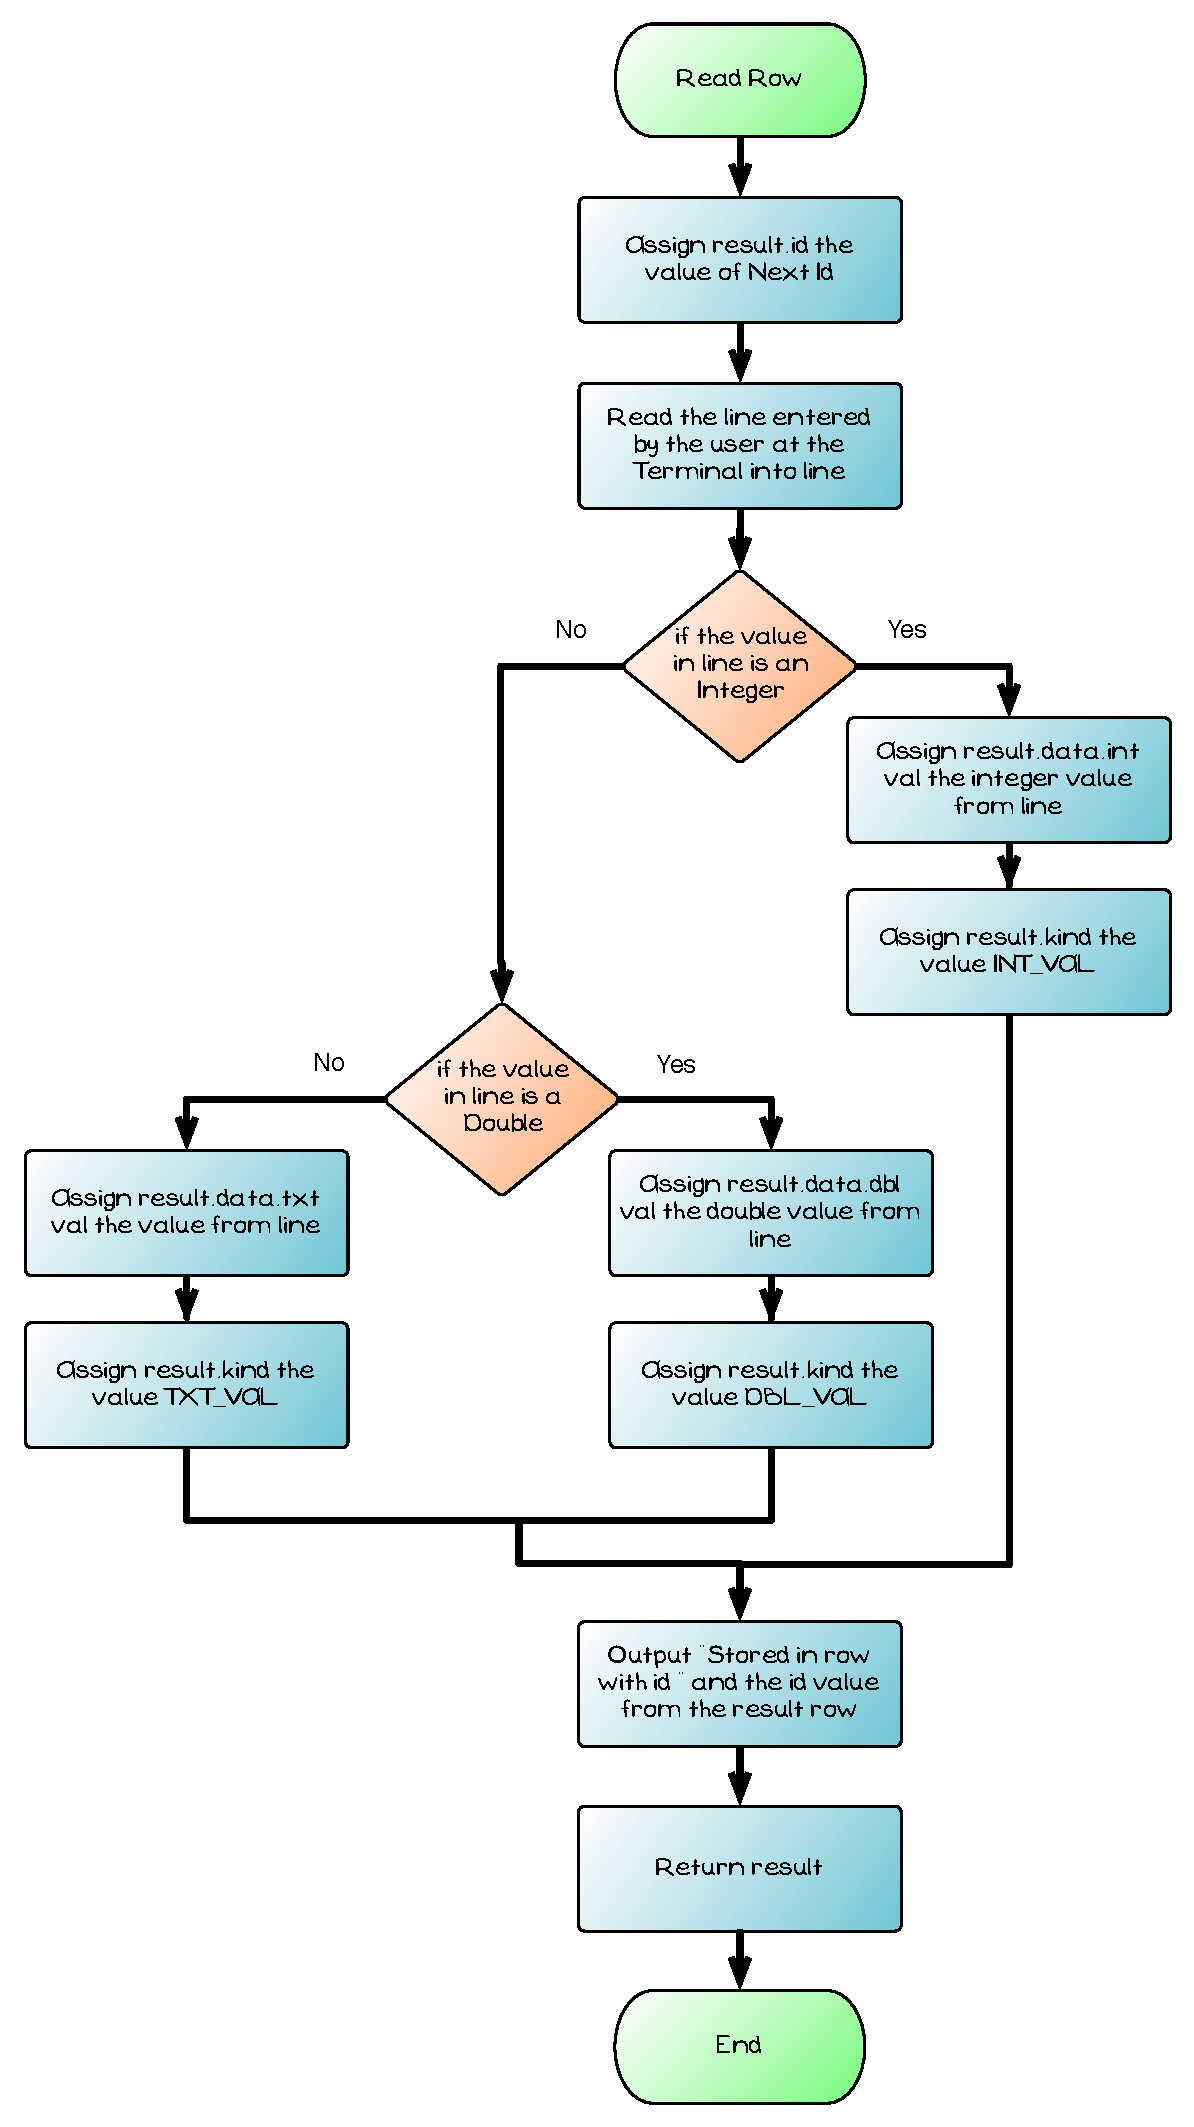
\includegraphics[width=0.80\textwidth]{./topics/type-decl/diagrams/ReadRowFlow} 
   \caption{Flowchart for \texttt{Read Row}, from \fref{fig:read-row-flow}}
   \label{fig:read-row-flow-understanding}
\end{figure}

\clearpage
\subsubsection{Code is loaded for Small DB} % (fold)
\label{ssub:code_is_loaded_for_small_db}

When the program starts its code is loaded into memory and its \texttt{main} procedure is started.

\begin{figure}[htbp]
   \centering
   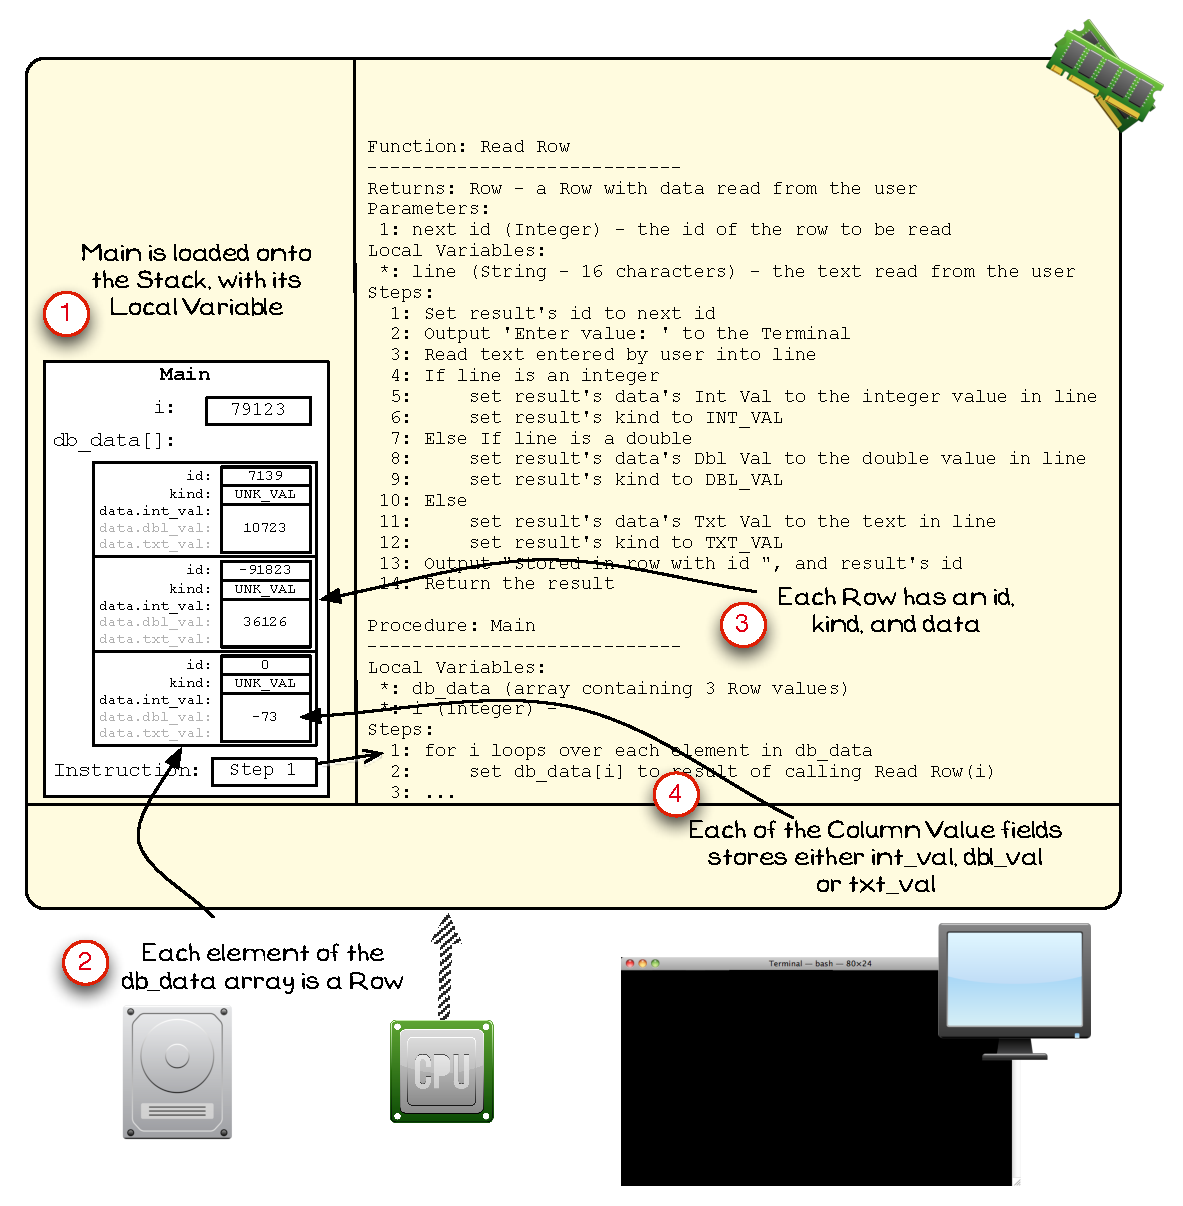
\includegraphics[width=0.9\textwidth]{./topics/type-decl/images/ReadRow1} 
   \caption{When the program starts \texttt{Main} allocates space for its local variables, including the array}
   \label{fig:read-row-vis-1}
\end{figure}

\mynote{
\begin{itemize}
  \item In \fref{fig:read-row-vis-1} the indicated areas show the following:
  \begin{enumerate}
    \item The Program starts and \texttt{Main} is loaded onto the stack, allocating space for its local variables.
    \item The \texttt{db\_data} array is allocated space to store its values. Each element of the array has the fields declared in the \texttt{Row} record structure.
    \item Each \texttt{Row} has an \texttt{id}, \texttt{kind}, and \texttt{data} value.
    \item Each of these \texttt{data} values has \emph{either} a \texttt{int\_val}, a \texttt{dbl\_val} or a \texttt{txt\_val}.
  \end{enumerate}
  \medskip
  \item Notice that the values in the array are allocated next to each other.
  \item In the illustration the \texttt{Row}'s \texttt{data} field will have only one of its fields highlighted, indicating which field is currently stored in the union.
\end{itemize}
}

% subsubsection code_is_loaded_for_small_db (end)

\clearpage
\subsubsection{\texttt{Read Row} is called to read in row with id 0} % (fold)
\label{ssub:read_row_is_called_to_read_in_row_with_id_0}

The \texttt{Read Row} function is called to read a \texttt{row} value from the user. This will check what the user has entered and store an appropriate value in the \texttt{Row} it returns.

\begin{figure}[htbp]
   \centering
   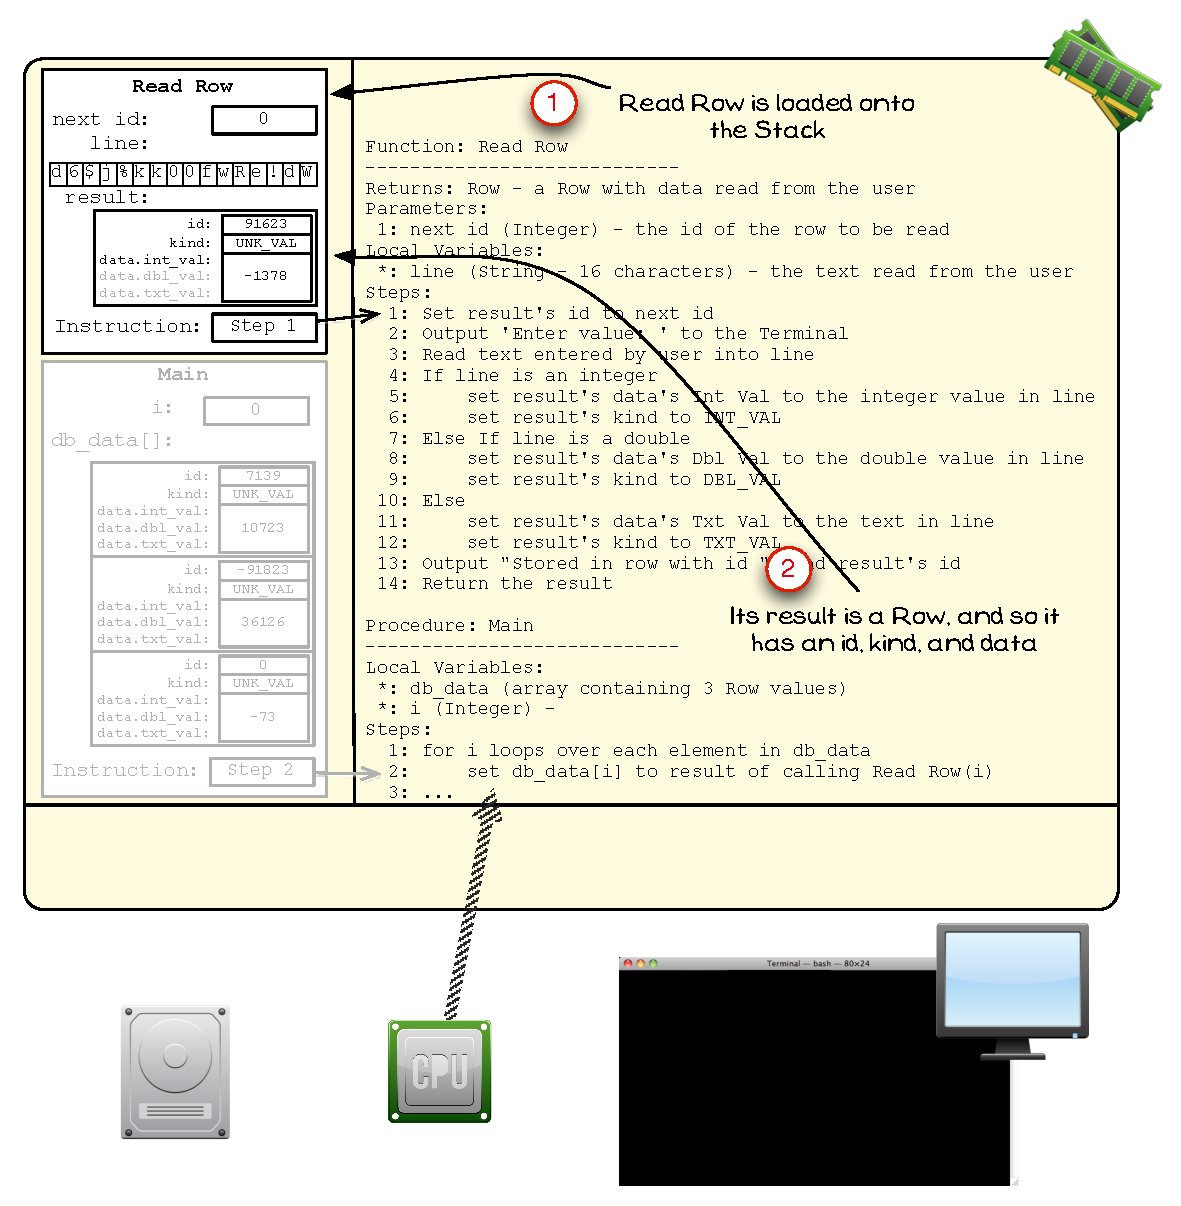
\includegraphics[width=\textwidth]{./topics/type-decl/images/ReadRow2} 
   \caption{At step 2 \texttt{Main} calls \texttt{Read Row}, getting it to read in the $i^{th}$ row from the user}
   \label{fig:read-row-vis-2}
\end{figure}

\mynote{
\begin{itemize}
  \item In \fref{fig:read-row-vis-2} the indicated areas show the following:
  \begin{enumerate}
    \item When \texttt{Read Row} is called it is allocated space on the stack.
    \item \texttt{Read Row} will be returning a \texttt{Row} value, so its result will have \texttt{id}, \texttt{kind}, and \texttt{data} values as these are what is specified in the \texttt{Row} record's definition.
  \end{enumerate}
  \medskip
  \item Each row will have the same kind of data stored within it. The details of this are specified in the \texttt{Row} record's definition.
\end{itemize}
}

% subsubsection read_row_is_called_to_read_in_row_with_id_0 (end)

\clearpage
\subsubsection{Step 1 stores the value 0 in \texttt{result}'s \texttt{id} field} % (fold)
\label{ssub:step_1_stores_the_value_0_in_result_s_id_field}

\begin{figure}[htbp]
   \centering
   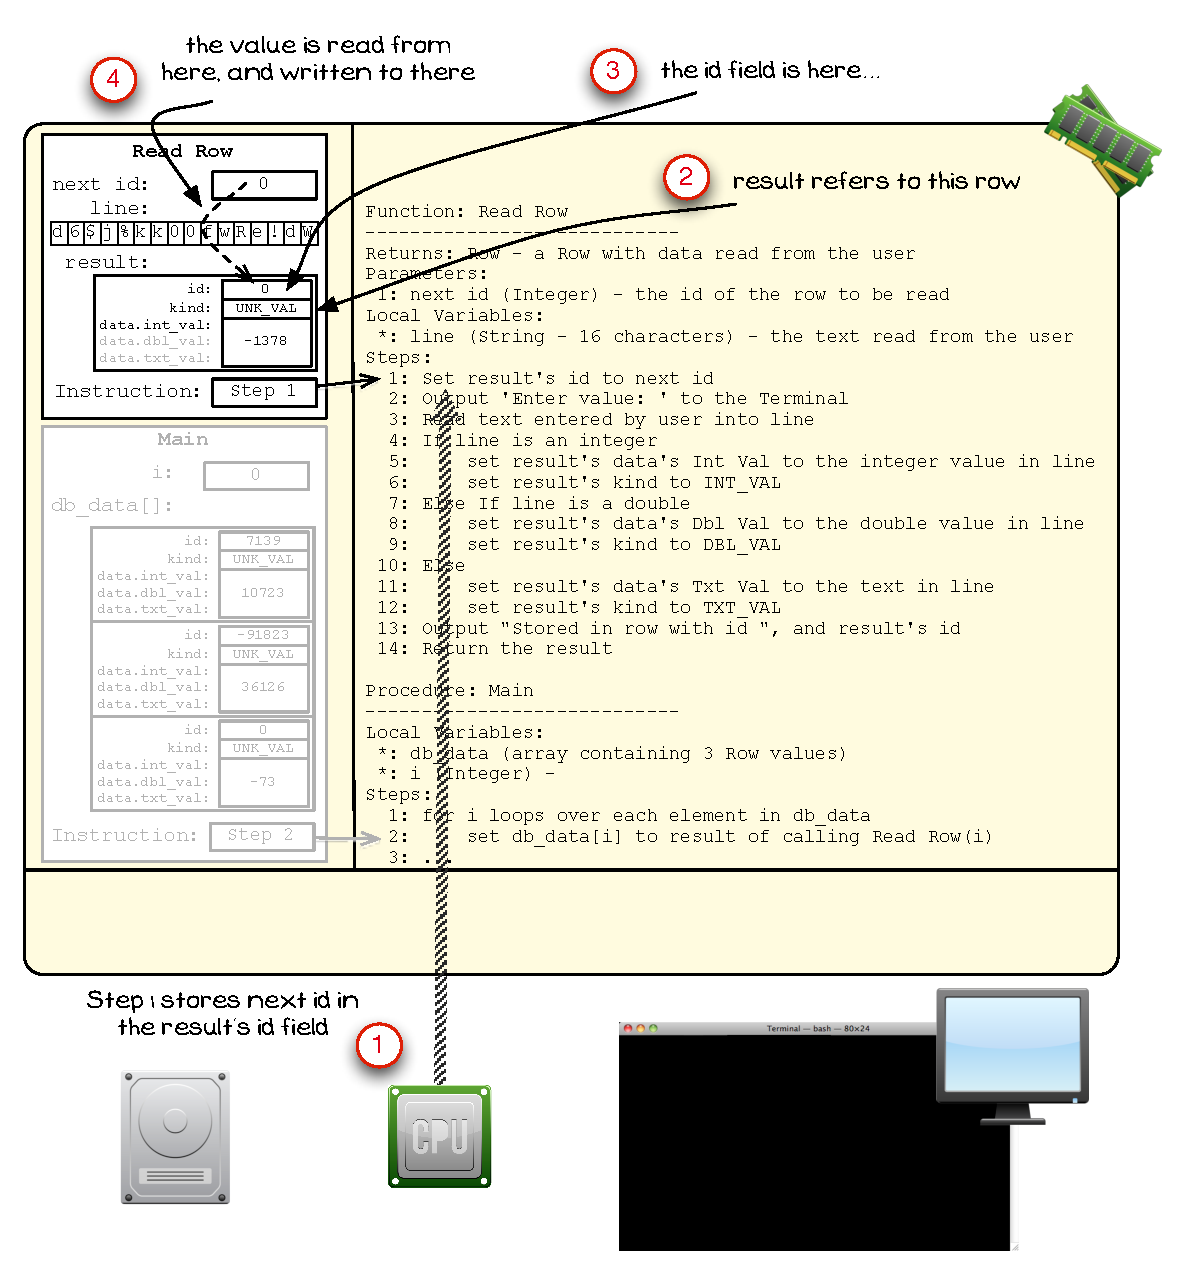
\includegraphics[width=0.98\textwidth]{./topics/type-decl/images/ReadRow3} 
 \caption{Step 1 of \texttt{Read Row} stores a value in \texttt{result}'s id}
 \label{fig:read-row-vis-3}
\end{figure}

\mynote{
\begin{itemize}
\item In \fref{fig:read-row-vis-3} the indicated areas show the following:
\begin{enumerate}
  \item Step 1 of \texttt{Read Row} assigns a value to \texttt{result.id}.
  \item In this code \texttt{result} refers to this variable in \texttt{Read Row}.
  \item The \texttt{id} part then refers to this field.
  \item As a result the value from the \texttt{next id} parameter is read, and its value is assigned to \texttt{result.id}.
\end{enumerate}
\medskip
\item Each part of \texttt{result.id} refers to a different kind of data.
\item \texttt{result} is a row, this has \texttt{id}, \texttt{kind}, and \texttt{data} fields.
\item \texttt{result.id} is an \texttt{Integer}, it is the id field of the \texttt{result Row}.
\end{itemize}
}

% subsubsection step_1_stores_a_value_in_result_s_id_field (end)

\clearpage
\subsubsection{A double value is entered by the user} % (fold)
\label{ssub:a_double_value_is_entered_by_the_user}

\begin{figure}[htbp]
   \centering
   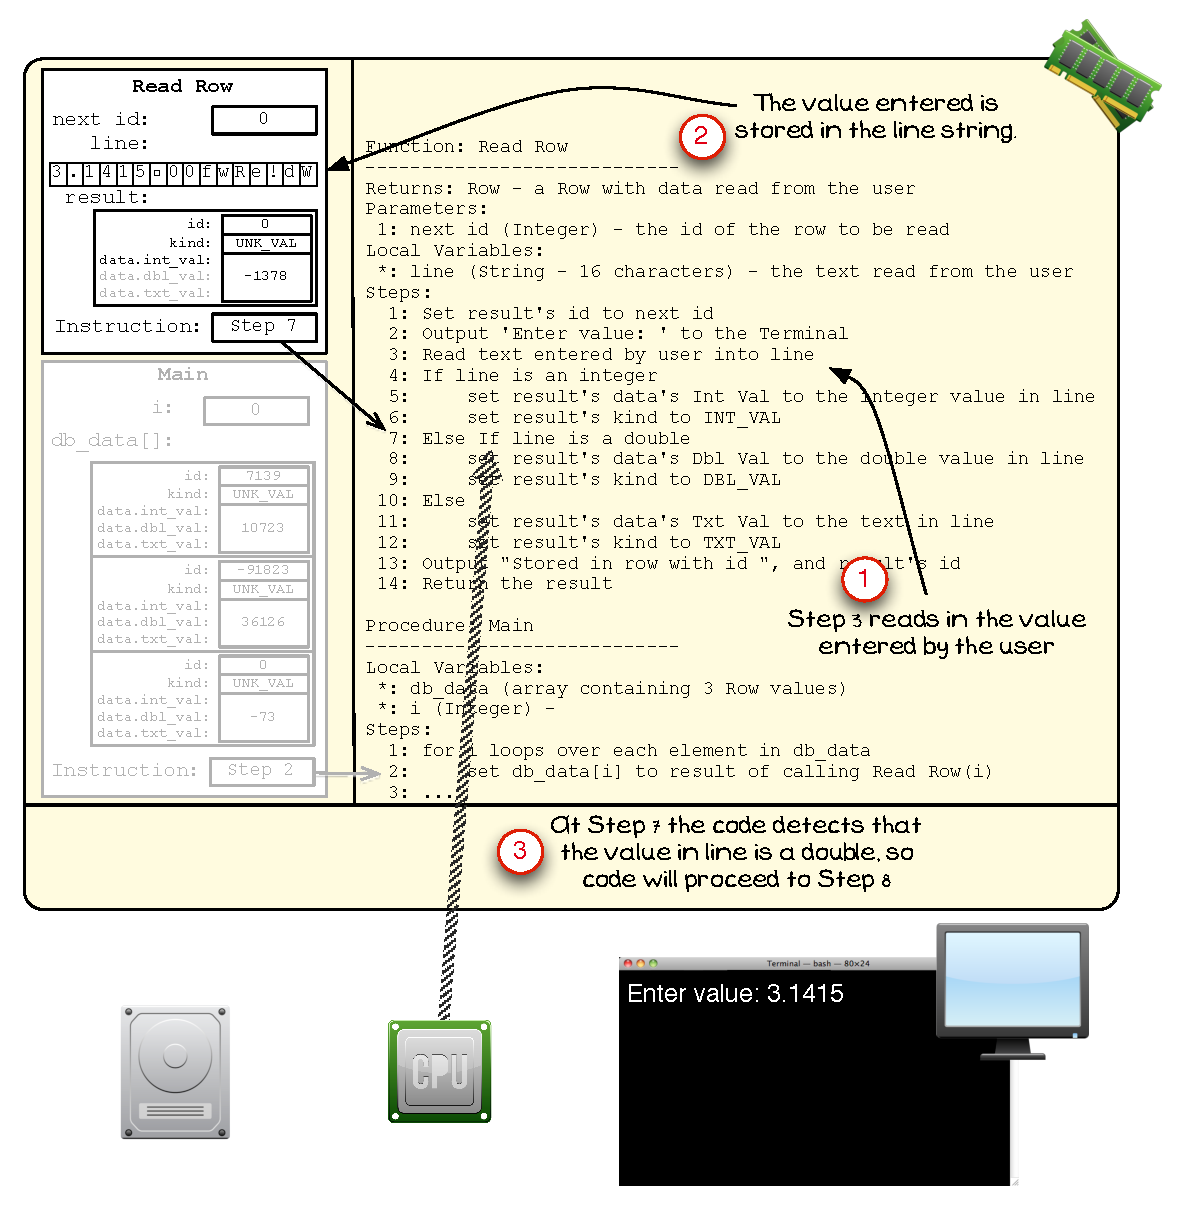
\includegraphics[width=0.98\textwidth]{./topics/type-decl/images/ReadRow4} 
 \caption{A double value is entered by the user, so the code must store the double in the row}
 \label{fig:read-row-vis-4}
\end{figure}

\mynote{
\begin{itemize}
\item In \fref{fig:read-row-vis-4} the indicated areas show the following:
\begin{enumerate}
  \item At Step 3 the computer reads the text entered by the user.
  \item The value read is stored in the \texttt{line} variable.
  \item At Step 7 the code determines that the data is a double, and execution will proceed to step 8.
\end{enumerate}
\medskip
\end{itemize}
}

% subsubsection a_double_value_is_entered_by_the_user (end)

\clearpage
\subsubsection{The double data is stored in the row} % (fold)
\label{ssub:the_double_data_is_stored_in_the_row}

\begin{figure}[htbp]
   \centering
   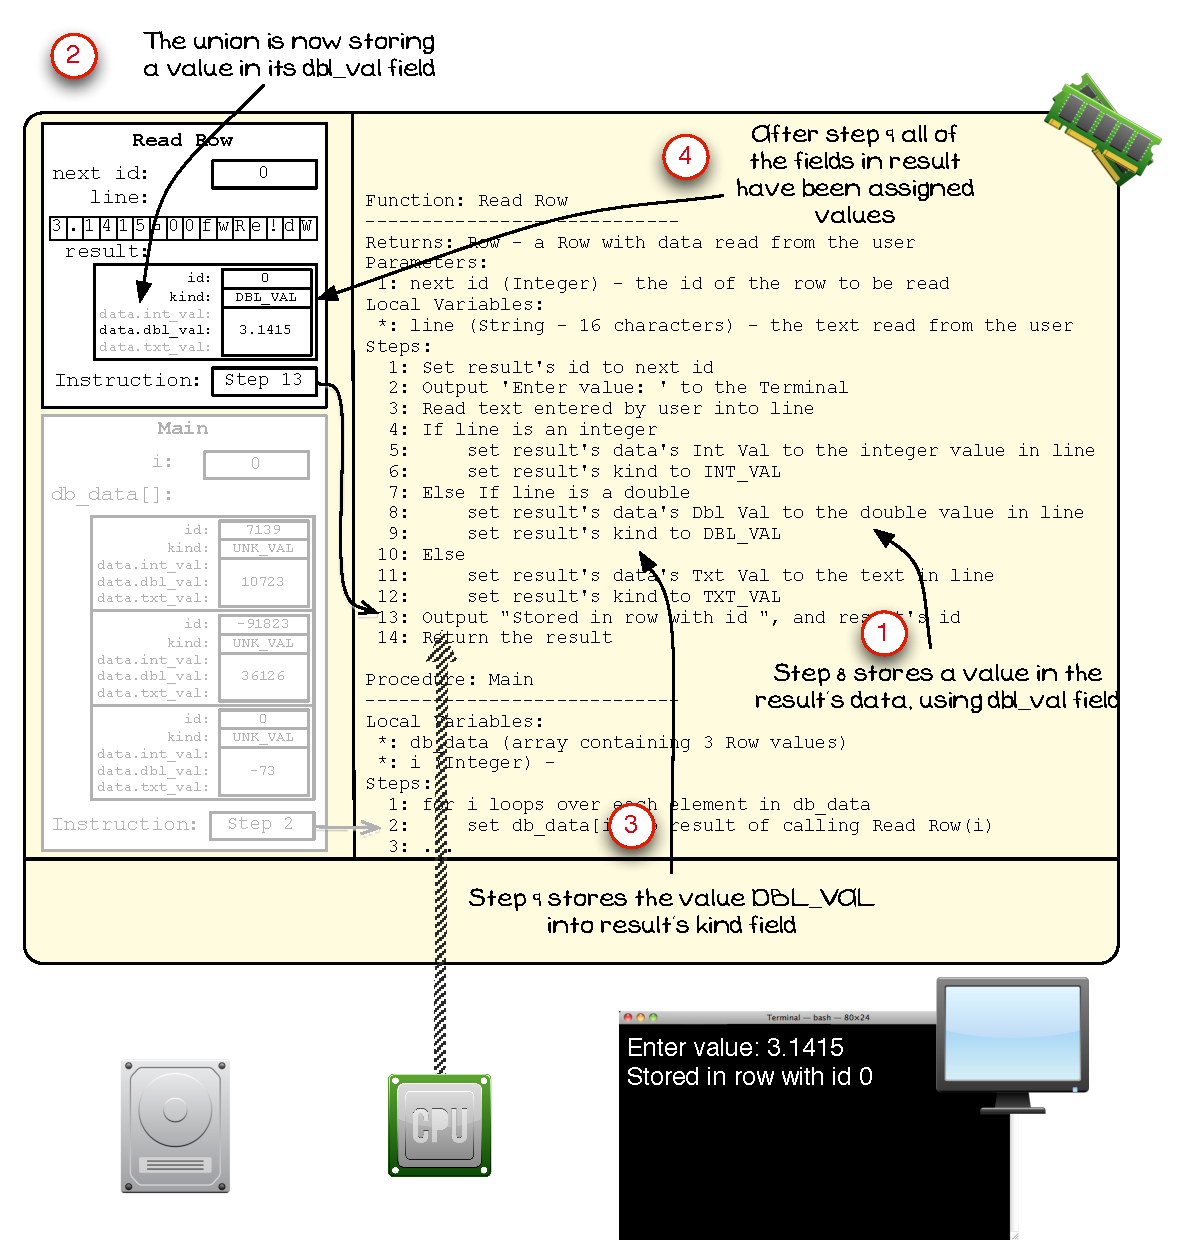
\includegraphics[width=\textwidth]{./topics/type-decl/images/ReadRow5} 
 \caption{A double value is entered by the user, so the code must store the double in the row}
 \label{fig:read-row-vis-5}
\end{figure}

\mynote{
\begin{itemize}
\item In \fref{fig:read-row-vis-5} the indicated areas show the following:
\begin{enumerate}
  \item Step 8 of \texttt{Read Row} stores the double value entered by the user into the \texttt{dbl\_val} field of the \texttt{data} field of the \texttt{result Row}.
  \item Notice that the union is now shown as storing a value in its \texttt{dbl\_val} field.
  \item Step 9 stores the \texttt{DBL\_VAL} value in the \texttt{kind} field of the \texttt{result Row}. This is one of the values from the \texttt{Data Kind} enumeration.
  \item At this point all of the fields of \texttt{result} have been assigned values.
\end{enumerate}
\medskip
\end{itemize}
}

% subsubsection the_double_data_is_stored_in_the_row (end)

\clearpage
\subsubsection{The \texttt{result} row is returned to \texttt{Main}} % (fold)
\label{ssub:the_result_row_is_returned_to_main}

\begin{figure}[htbp]
   \centering
   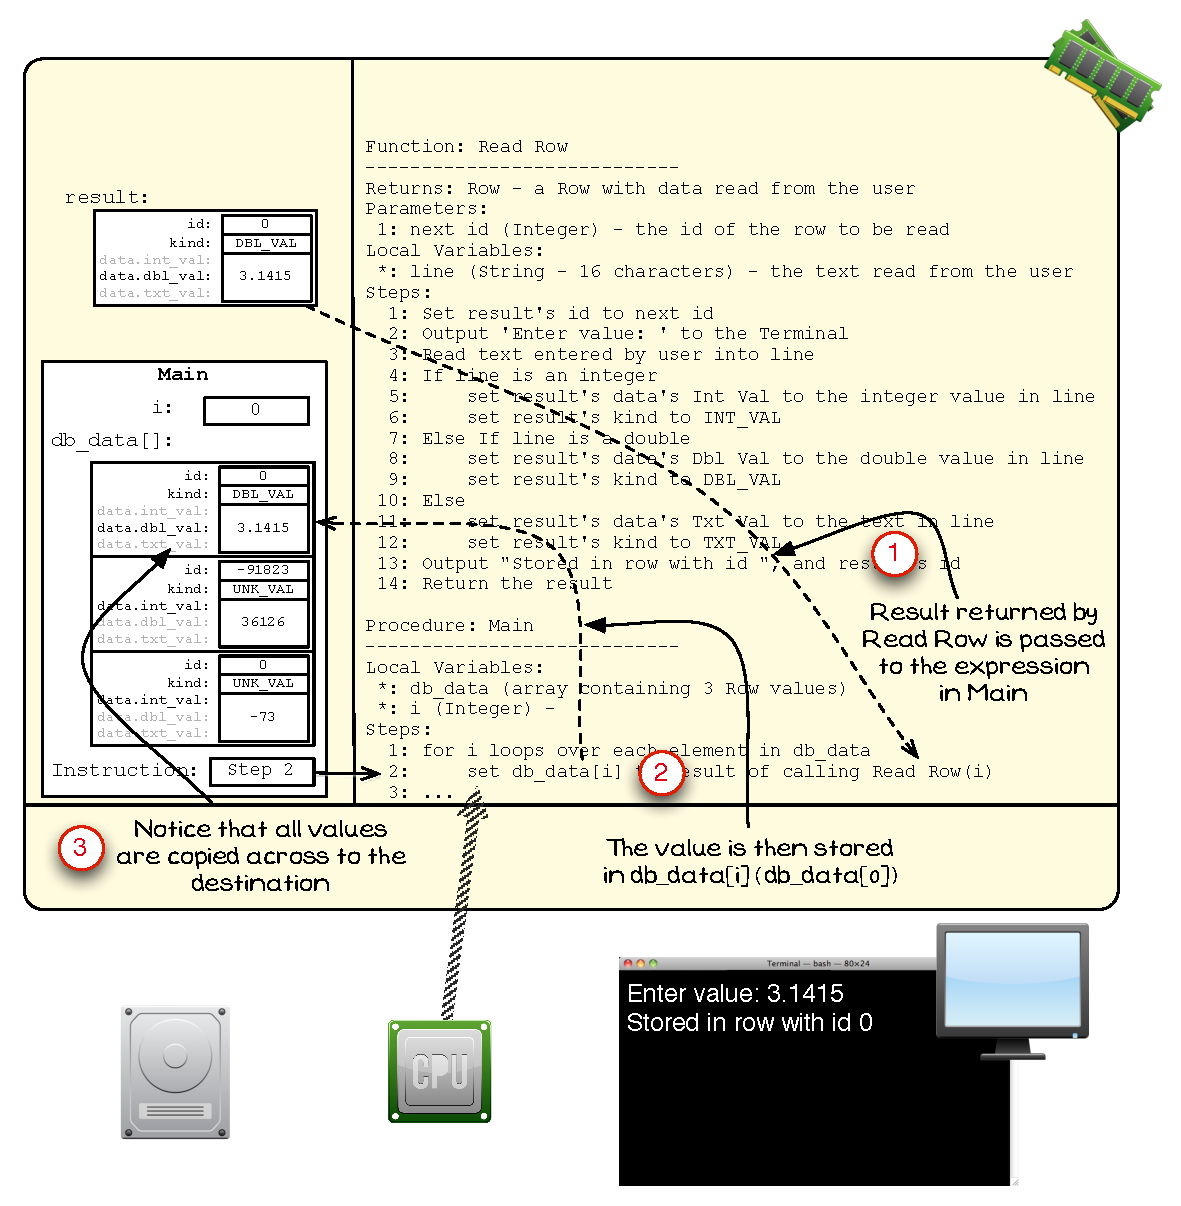
\includegraphics[width=\textwidth]{./topics/type-decl/images/ReadRow6} 
 \caption{The \texttt{result Row} is returned to \texttt{Main}}
 \label{fig:read-row-vis-6}
\end{figure}

\mynote{
\begin{itemize}
\item In \fref{fig:read-row-vis-6} the indicated areas show the following:
\begin{enumerate}
  \item At the end of \texttt{Read Row} the \texttt{result Row} is returned to \texttt{Main}.
  \item In \texttt{Main} the value is used in an assignment statement, that assigns it to the $i^{th}$ value in the \texttt{db\_data} array. As \texttt{i} is currently 0, this stores the \textbf{entire} row in \texttt{dd\_data[0]}.
  \item When this assignment occurs all of the data from the \texttt{result} of \texttt{Read Row} is copied into \texttt{db\_data[0]}.
\end{enumerate}
\medskip
\item With Records and Unions you can read/write to individual fields using the dot notation, or you can access the entire record.
\end{itemize}
}


% subsubsection the_result_row_is_returned_to_main (end)

\clearpage
\subsubsection{This process is repeated for each element of the array} % (fold)
\label{ssub:this_process_is_repeated_for_each_element_of_the_array}

\begin{figure}[htbp]
   \centering
   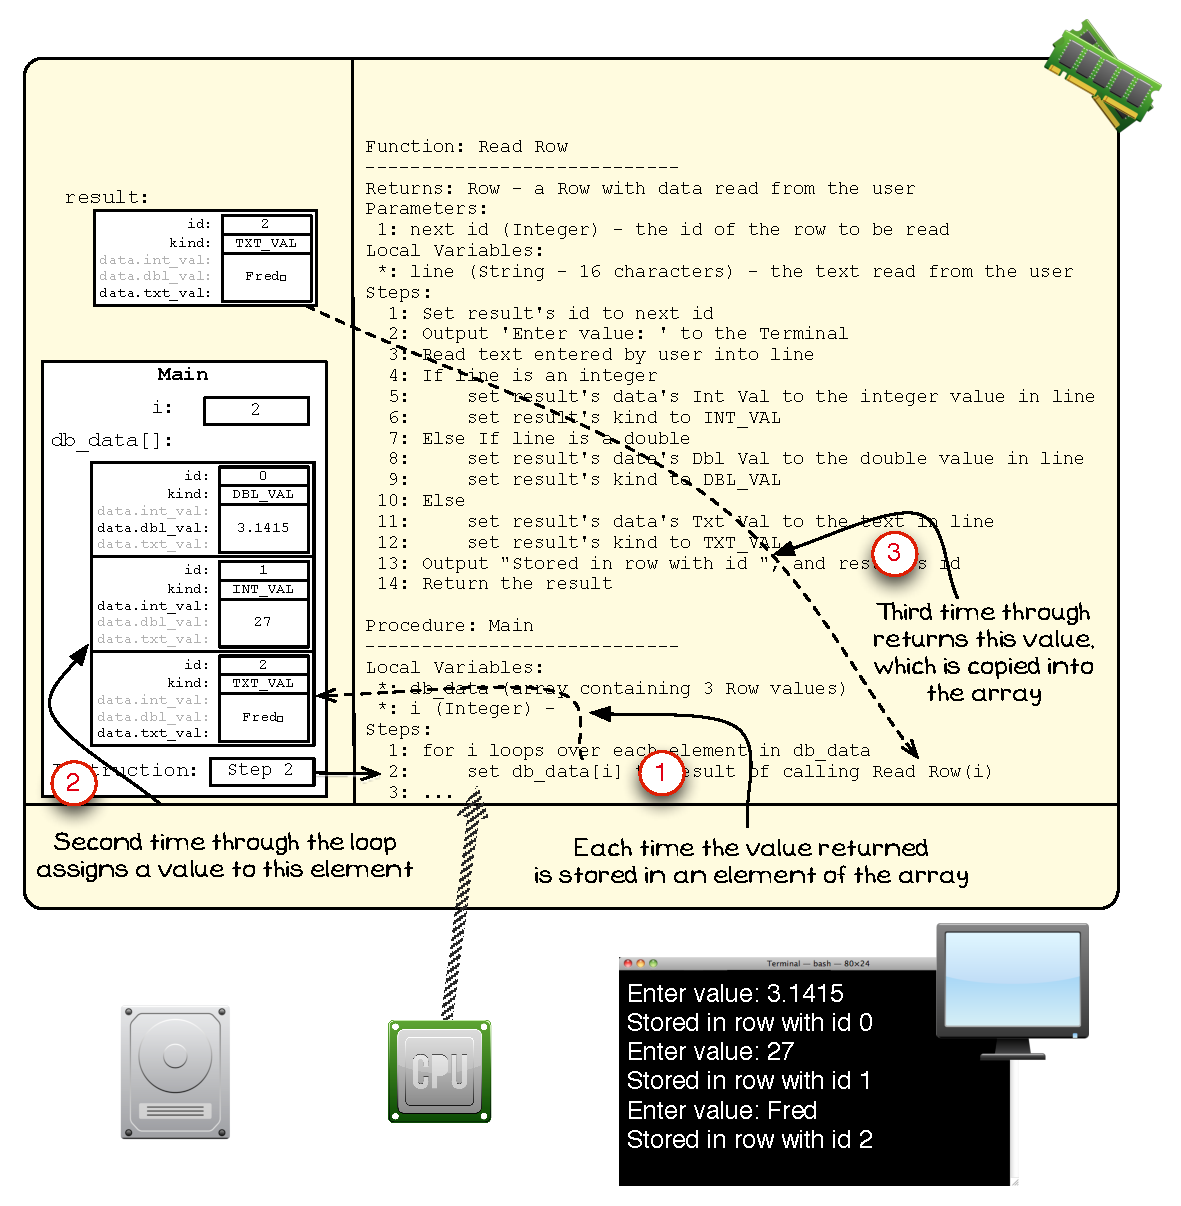
\includegraphics[width=0.92\textwidth]{./topics/type-decl/images/ReadRow7} 
 \caption{The for loop ensures that a \texttt{Row} value is read in for each element of the array}
 \label{fig:read-row-vis-7}
\end{figure}

\mynote{
\begin{itemize}
\item In \fref{fig:read-row-vis-7} the indicated areas show the following:
\begin{enumerate}
  \item Each time through the loop the value is written to an element in the array. This is showing the last iteration where \texttt{i} is 2.
  \item The second time this loop was executed the user entered an integer value, this is now stored in the second element of the array.
  \item The third time through the loop, the result returned is storing a string value. This is returned to \texttt{Main}, and then stored in the \texttt{db\_data} array.
\end{enumerate}
\medskip
\item Notice that there is only ever one value in each \texttt{Row}'s \texttt{data}. This is a \textbf{union}, and only stores one of its field values.
\item See how the enumeration values indicate the field the data has been stored in. This is why the enumeration's constants were named in a similar\footnote{They could have been named anything, but this reflects their purpose well.} way to the union's fields.
\end{itemize}
}

% subsubsection this_process_is_repeated_for_each_element_of_the_array (end)

% subsection understanding_read row (end)
\clearpage
\subsection{Understanding \texttt{Print Row}} % (fold)
\label{sub:understanding_print row}

\texttt{Print Row} is the other key piece of logic in the Small DB program. This procedure outputs the values read from the user to the Terminal. It uses the data stored in the \texttt{Row}'s fields to determine how this value is output, and how the data can be read. The flowchart of this logic is shown in \fref{fig:print-row-flow-understanding}.

\begin{figure}[htbp]
   \centering
   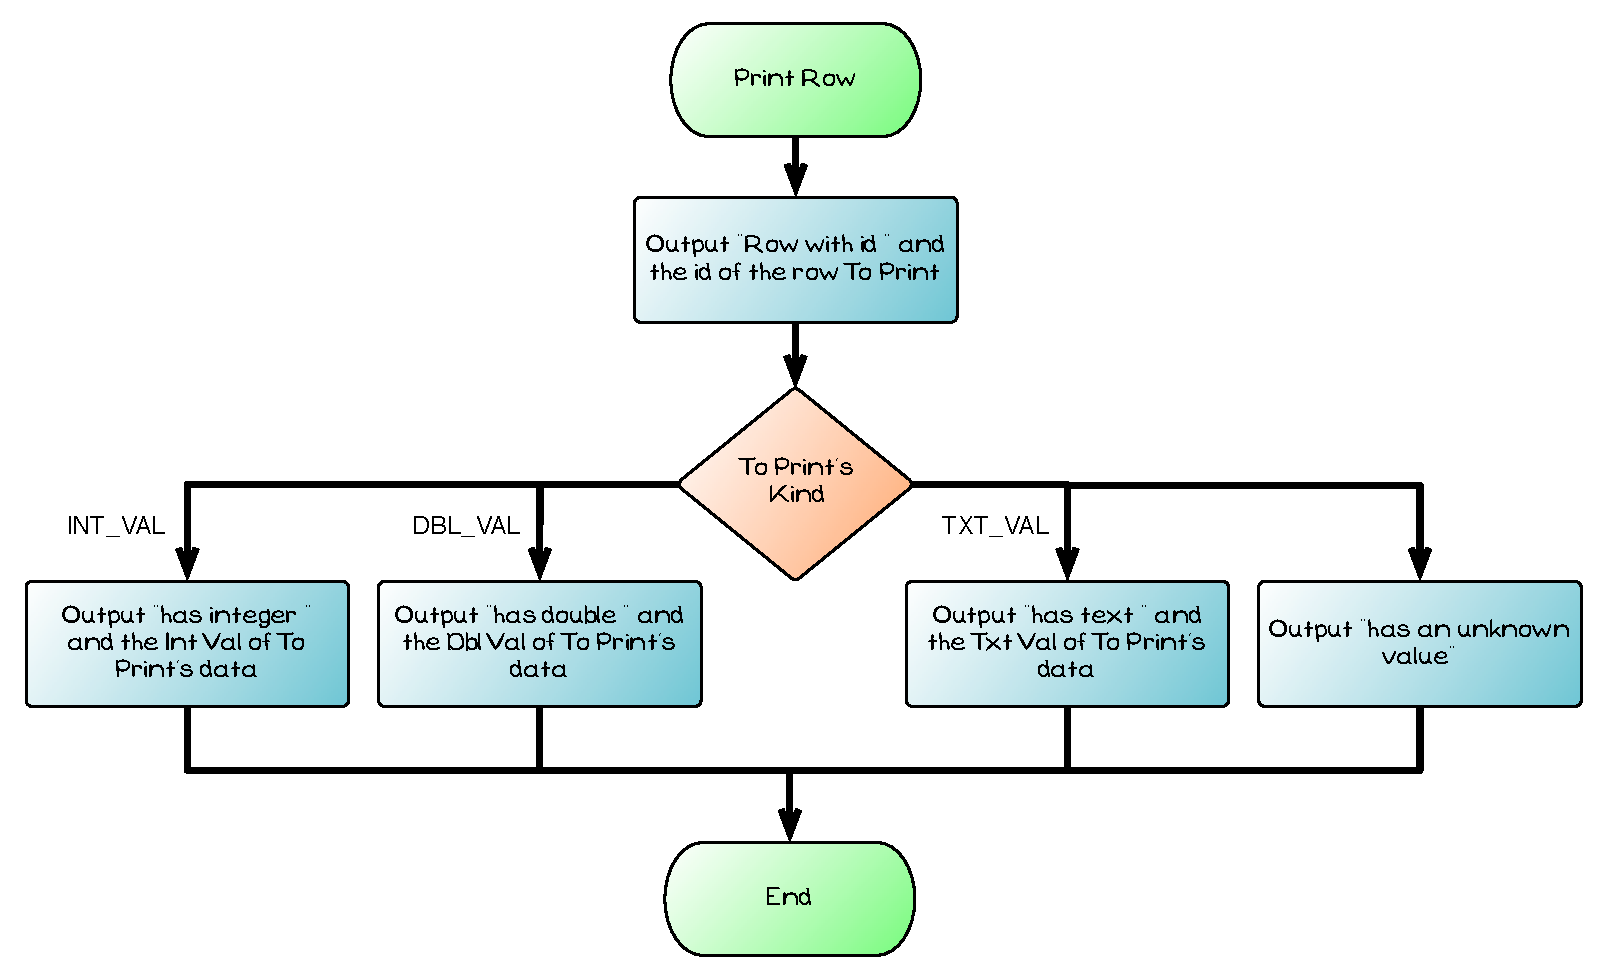
\includegraphics[width=\textwidth]{./topics/type-decl/diagrams/PrintRowFlow} 
   \caption{Flowchart of the steps needed to print a \texttt{Row} to the Terminal, from \fref{fig:print-row-flow}}
   \label{fig:print-row-flow-understanding}
\end{figure}

Within \texttt{Main}, \texttt{Print Row} is called once for each \texttt{Row} in the \texttt{db\_data} array. The following illustrations demonstrate the third and final call to \texttt{Print Row}.

The illustrations will show the following:
\begin{enumerate}
  \item \nameref{ssub:print_row_is_called_for_each_element_in_the_array}
  \item \nameref{ssub:the_text_value_is_output_to_the_terminal}
\end{enumerate}

You can use these details to determine how the other data was written to the Terminal. 

\clearpage
\subsubsection{\texttt{Print Row} is called for each element in the array} % (fold)
\label{ssub:print_row_is_called_for_each_element_in_the_array}

This illustration starts part way through the third call to \texttt{Print Row}. At this stage the first two rows have been output to the Terminal, as has the \texttt{id} of the third \texttt{Row}.

\begin{figure}[htbp]
   \centering
   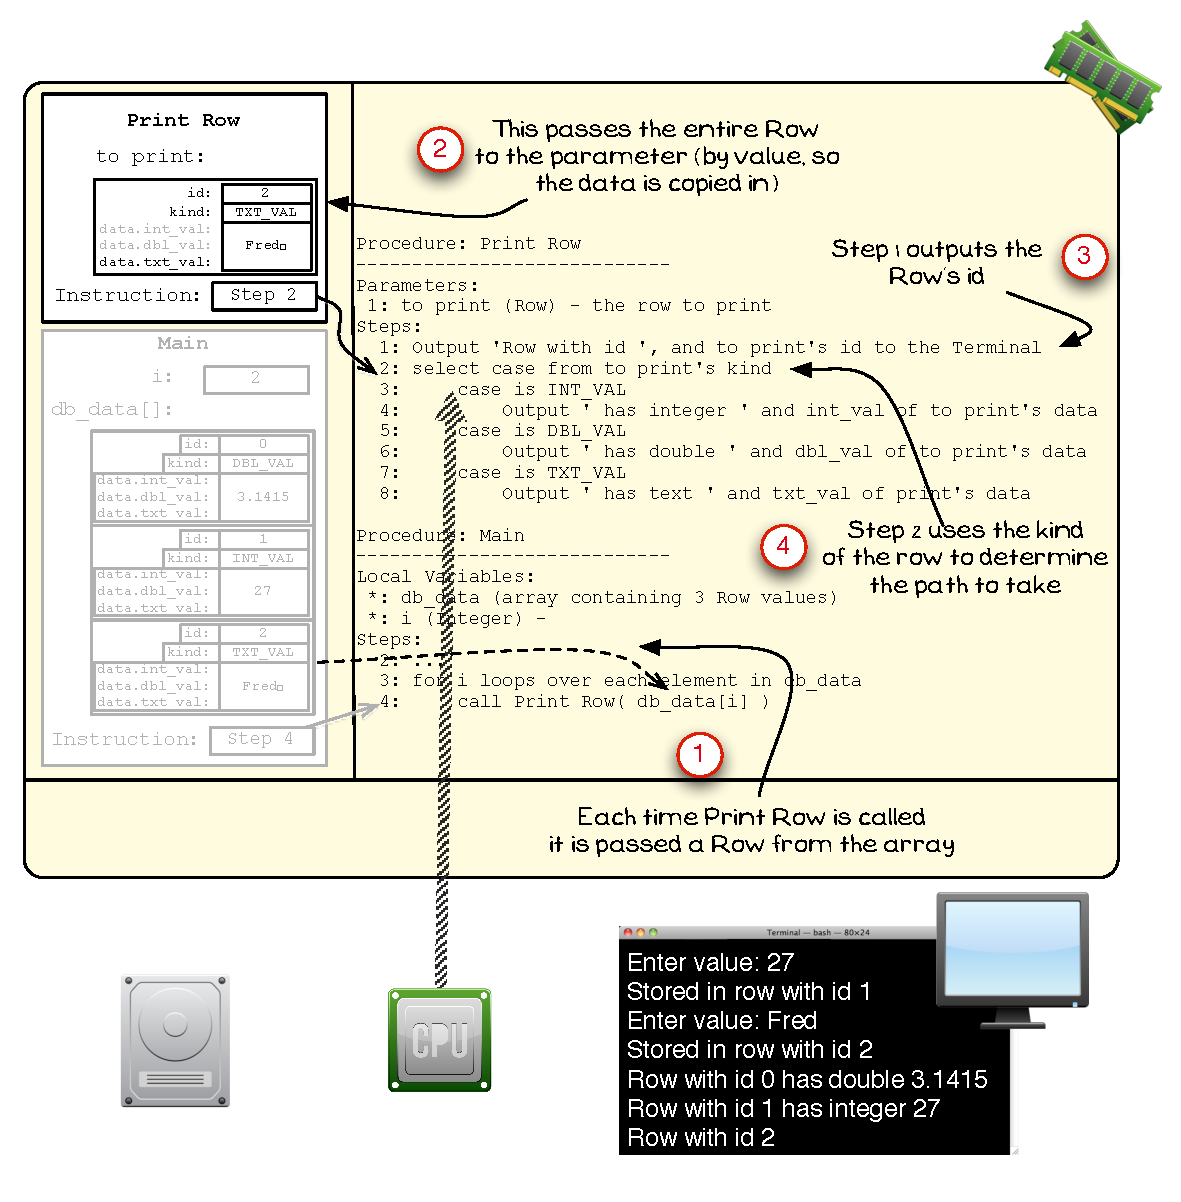
\includegraphics[width=0.92\textwidth]{./topics/type-decl/images/PrintRow1} 
 \caption{\texttt{Print Row} is called for each of the \texttt{Row} elements in \texttt{db\_data}}
 \label{fig:print-row-vis-1}
\end{figure}

\mynote{
\begin{itemize}
\item In \fref{fig:print-row-vis-1} the indicated areas show the following:
\begin{enumerate}
  \item This is the third call to \texttt{Print Row}. Each time this procedure is called it receives a copy of the data from the element passed to it.
  \item The parameter is a copy of the data from the array element.
  \item The first action in \texttt{Print Row} is to output the \texttt{id} value from the \texttt{to print} \texttt{Row}.
  \item The illustration is showing the computer at the stage where it is reading \texttt{to print}'s \texttt{kind} to determine which path to take. As \texttt{to print}'s \texttt{kind} is currently \texttt{TXT\_VAL} it will take the path at Step 8.
\end{enumerate}
\medskip
\item The case statement will allow the code to output the message that matches the kind of data stored in \texttt{to print}.
\end{itemize}
}

% subsubsection print_row_is_called_for_each_element_in_the_array (end)

\clearpage
\subsubsection{The text value is output to the Terminal} % (fold)
\label{ssub:the_text_value_is_output_to_the_terminal}

\begin{figure}[htbp]
   \centering
   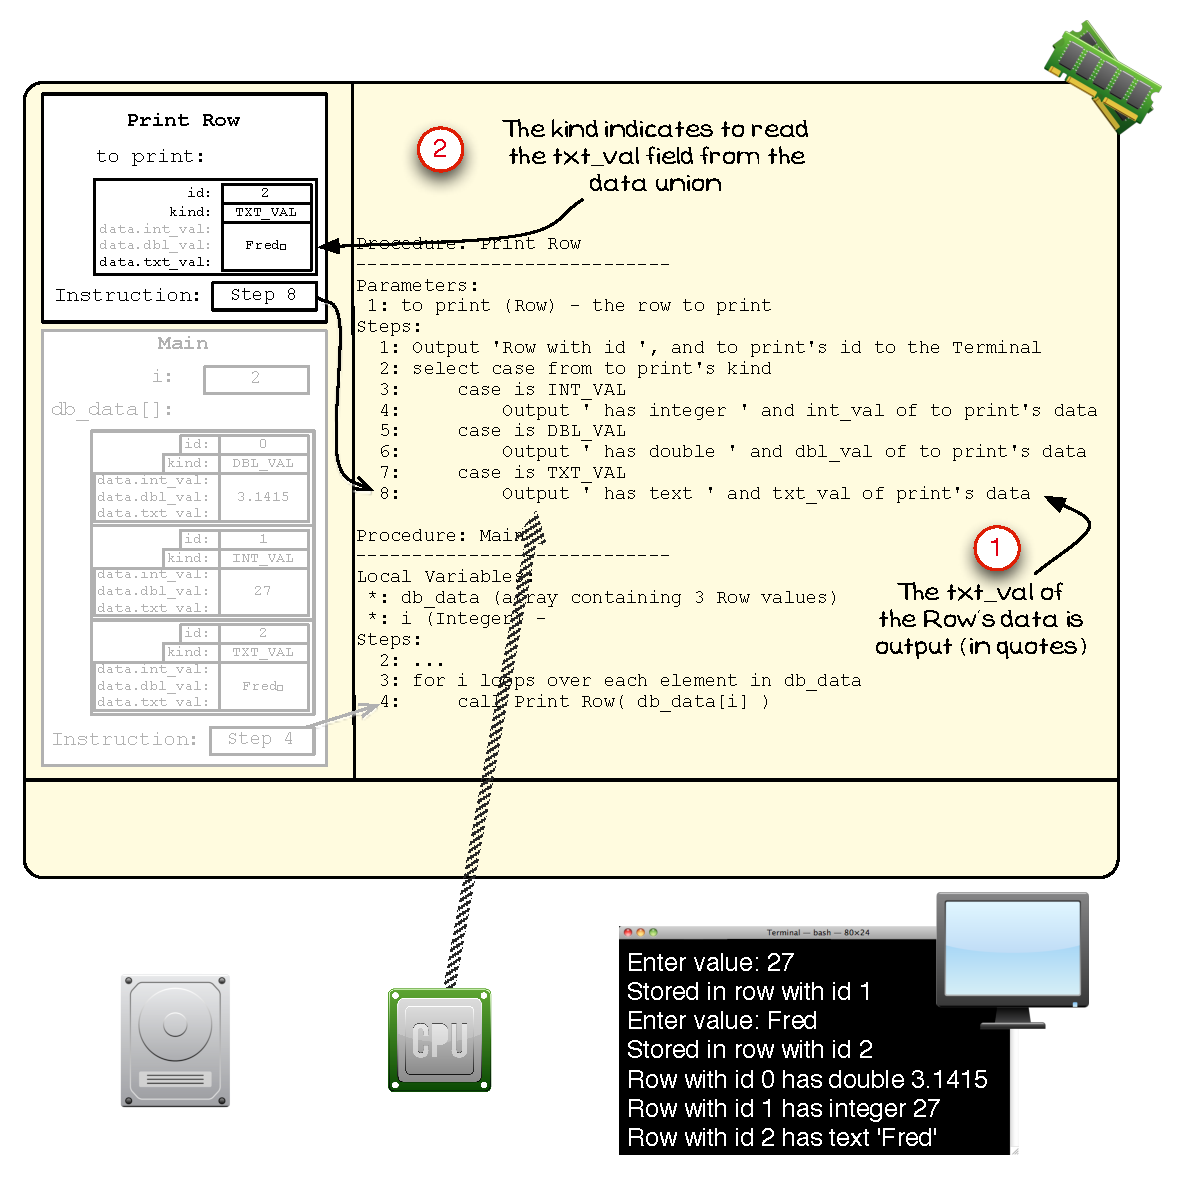
\includegraphics[width=0.91\textwidth]{./topics/type-decl/images/PrintRow2} 
 \caption{\texttt{Print Row} is called for each of the \texttt{Row} elements in \texttt{db\_data}}
 \label{fig:print-row-vis-2}
\end{figure}

\mynote{
\begin{itemize}
\item In \fref{fig:print-row-vis-2} the indicated areas show the following:
\begin{enumerate}
  \item Step 8 reads the \texttt{txt\_val} field of \texttt{to print}'s \texttt{data} field. This reads the text value from within that field, and this is output to the Terminal.
  \item The \texttt{kind} field was used to determine which field to read from the union.
\end{enumerate}
\smallskip
\item In this example the record, union, and enumeration are all working together to enable the required functionality.
\item Without the enumeration it would not be possible to determine which field to read from the union. Reading any of the fields on the union would return data, but only the field that was written to can be relied about to have a meaningful value.
\item Without the union you would need to waste space storing all three data values, but only ever using one.
\item Without the record it would be hard to relate the values stored within a single \texttt{Row}. The row only existed because of the record's declaration.
\item Back in \texttt{Main}, the array allows you to store multiple of these values. 
\end{itemize}
}


% subsubsection the_text_value_is_output_to_the_terminal (end)


% subsection understanding_print row (end)


% section understanding_custom_types (end)

% ============
% = Examples =
% ============
\clearpage
\section{Example Custom Types} % (fold)
\label{sec:example_custom_types}

\subsection{Lights} % (fold)
\label{sub:lights}

This example draws three light bulbs to the screen. These lights can be clicked to turn them on and off. The code includes the declaration of a record/structure and an enumeration.

\begin{figure}[h]
   \centering
   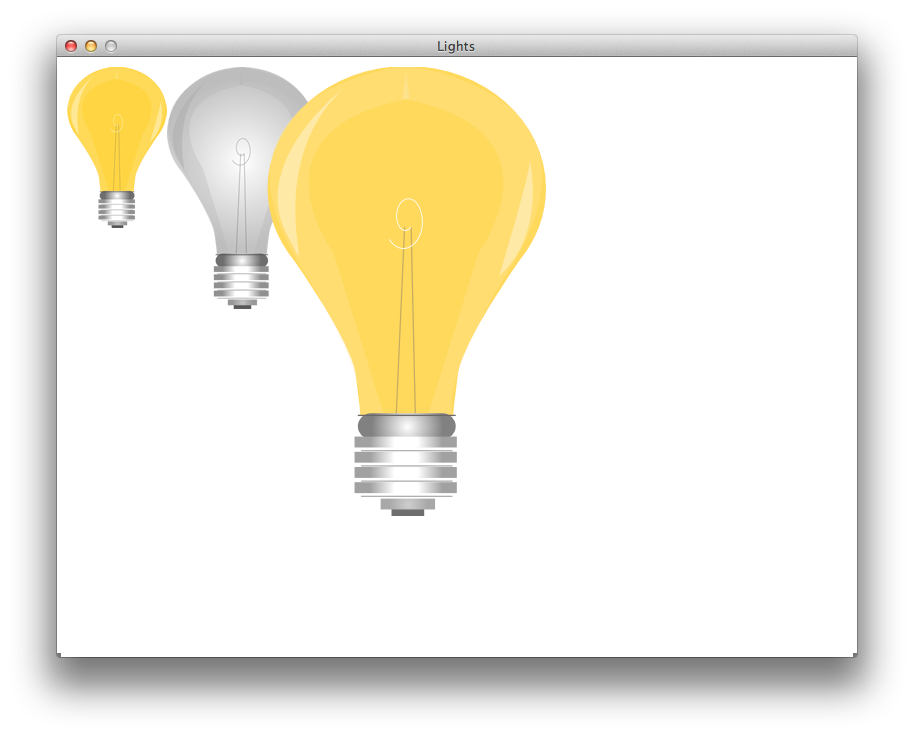
\includegraphics[width=0.8\textwidth]{./topics/type-decl/examples/Lights.png} 
   \caption{Example execution of the Lights program}
   \label{fig:lights-img}
\end{figure}

\clearpage

\cppsection{\ccode{cpplst:lights}{Lights code in C++, continues in \lref{cpplst:lights1} }{topics/type-decl/examples/lights.cpp}}

\cppsection{\ccode{cpplst:lights1}{Lights code in C++, continues in \lref{cpplst:lights2} }{topics/type-decl/examples/lights1.cpp}}

\cppsection{\ccode{cpplst:lights2}{Lights code in C++, continues in \lref{cpplst:lights3} }{topics/type-decl/examples/lights2.cpp}}

\cppsection{\ccode{cpplst:lights3}{Last of the Lights code in C++}{topics/type-decl/examples/lights3.cpp}}

\passection{\pascode{plst:lights}{Lights code in Pascal, continues in \lref{plst:lights1} }{topics/type-decl/examples/Lights.pas}}

\passection{\pascode{plst:lights1}{Lights code in Pascal, continues in \lref{plst:lights2} }{topics/type-decl/examples/Lights1.pas}}

\passection{\pascode{plst:lights2}{Lights code in Pascal, continues in \lref{plst:lights3} }{topics/type-decl/examples/Lights2.pas}}

\passection{\pascode{plst:lights3}{Lights code in Pascal }{topics/type-decl/examples/Lights3.pas}}

% subsection lights (end)
\clearpage
\subsection{Shape Drawing} % (fold)
\label{sub:shape_drawing}

The Shape Drawing program allows the user to create simple shape drawings using circles, triangles, rectangles, and ellipses. 

\begin{figure}[h]
   \centering
   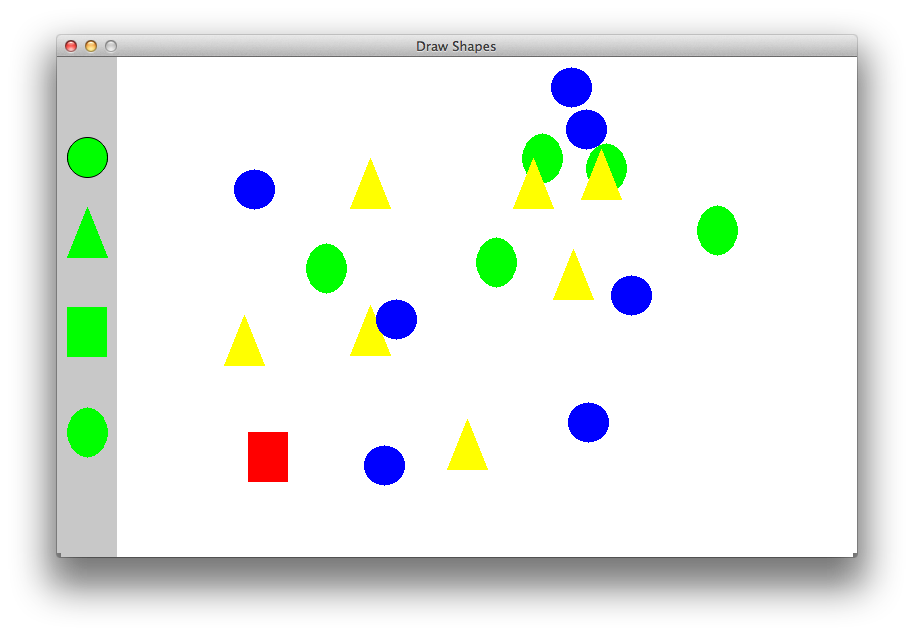
\includegraphics[width=\textwidth]{./topics/type-decl/examples/ShapeDrawing.png} 
   \caption{Example execution of the Shape Drawing program}
   \label{fig:shape-drawing-img}
\end{figure}

\clearpage

\cppsection{\ccode{cpplst:shape_drawing}{Shape Drawing code in C++, continues in \lref{cpplst:shape_drawing1} }{topics/type-decl/examples/shape_drawing.cpp}}

\cppsection{\ccode{cpplst:shape_drawing1}{Shape Drawing code in C++, continues in \lref{cpplst:shape_drawing2} }{topics/type-decl/examples/shape_drawing1.cpp}}

\cppsection{\ccode{cpplst:shape_drawing2}{Shape Drawing code in C++, continues in \lref{cpplst:shape_drawing3} }{topics/type-decl/examples/shape_drawing2.cpp}}

\cppsection{\ccode{cpplst:shape_drawing3}{Shape Drawing code in C++, continues in \lref{cpplst:shape_drawing4} }{topics/type-decl/examples/shape_drawing3.cpp}}

\cppsection{\ccode{cpplst:shape_drawing4}{Last of the Shape Drawing code in C++}{topics/type-decl/examples/shape_drawing4.cpp}}


\passection{\pascode{plst:shape_drawing}{Shape Drawing code in Pascal, continues in \lref{plst:shape_drawing1} }{topics/type-decl/examples/ShapeDrawing.pas}}

\passection{\pascode{plst:shape_drawing1}{Shape Drawing code in Pascal, continues in \lref{plst:shape_drawing2} }{topics/type-decl/examples/ShapeDrawing1.pas}}

\passection{\pascode{plst:shape_drawing2}{Shape Drawing code in Pascal, continues in \lref{plst:shape_drawing3} }{topics/type-decl/examples/ShapeDrawing2.pas}}

\passection{\pascode{plst:shape_drawing3}{Last Shape Drawing code in Pascal }{topics/type-decl/examples/ShapeDrawing2.pas}}


% subsection shape_drawing (end)

% section example_custom_types (end)


% =============
% = Exercises =
% =============
\clearpage
\section{Custom Type Exercises} % (fold)
\label{sec:custom_type_exercises}

Read over the concepts in this chapter and answer the following questions:
\begin{enumerate}
  \item What is a type?
  \item What is the relationship between a type and a value? 
  \item When you create your own type what have you created? A value, or something else?
  \item Why would you want to create your own type?
  \item What are the three main kinds of type you can create?
  \item What kind of data type(s) could you create to model the following in a program?
  \begin{enumerate}
    \item An address book, containing names, phone numbers, and email addresses.
    \item The kind of a `\emph{power up}' in a game, e.g. health pack, upgrade, bonus, etc.
    \item A field that is either an integer, a double, or some text.
    \item A button that has a location on the screen, a width and height, and some text that is drawn on the button.
  \end{enumerate}
  \item What is a record? What can it be used to model?
  \item What is an enumeration? What can it be used to model?
  \item What is a union? What can it be used to model?
  \item Why is it a good idea to use an enumeration in conjuncture with a union?
  \item Explain the different ways you can store/read a value when you are using a record.
  \item Explain the different ways you can store/read a value when you are using a enumeration.
  \item Explain the different ways you can store/read a value when you are using a union.
  \item Open one of your SwinGame projects and have a look in the \texttt{lib} folder. This folder contains a number of source code files used to access SwinGame functionality. Have a look in the \textbf{Types} file (types.c or sgTypes.pas), and examine the follow types. For each type write a short description of what it contains.
  \begin{enumerate}
    \item Rectangle
    \item Circle
    \item LineSegment
    \item Triangle
    \item Point 2D
    \item Vector
  \end{enumerate}
\end{enumerate}

\clearpage
Apply what you have learnt to the following tasks:

\begin{enumerate}
  \item Implement the Small DB program, including the support for the double data in the row.
\end{enumerate}

\bigskip

If you want to further your knowledge in this area you can try to answer the following questions. The answers to these questions will require you to think harder, and possibly look at other sources of information.

\begin{enumerate}
  \item Extend the Small DB program so that each `\emph{row}' has three `\emph{columns}'. Change the \texttt{Row Value} type to \texttt{Column Value} to better represent its purpose.
\end{enumerate}


% section custom_type_exercises (end)

% ===========
% = Project =
% ===========
% \clearpage
% \section{Custom Types in the Project} % (fold)
% \label{sec:custom_types_in_the_project}

% section custom_types_in_the_project (end)


% chapter more_data_types (end)